% main.tex - Laporan Akhir Project "Pemetaan Cepat Tutupan Lahan".
% Kompilasi dari folder laporan/:  latexmk -pdf main.tex   (atau pdflatex tiga kali)
% Gaya diambil dari template proposal (preamble.tex); isi tiap bab ada di bab/.
% Makro penanda \isi (teks merah, preamble.tex) menandai bagian yang belum diisi; PDF final tidak memuatnya lagi.
\documentclass[12pt,a4paper]{report}

% preamble.tex - gaya laporan, disalin dari main.tex template proposal
% (Proposal_Color_Quantizer.zip); satu-satunya perubahan: jarak sebelum judul bab (\titlespacing*{\chapter}).
% Tambahan khusus laporan ada di bagian paling bawah.
% Jangan menambah \usepackage: MiKTeX memakai AutoInstall, paket baru bisa terunduh diam-diam.

% ===================== PAKET =====================
\usepackage[a4paper,top=3cm,bottom=3cm,left=3cm,right=2.5cm]{geometry}
\usepackage[utf8]{inputenc}
\usepackage[T1]{fontenc}
\usepackage{mathptmx}
\renewcommand{\ttdefault}{lmtt}
\usepackage{textcomp}
\usepackage{graphicx}
\usepackage[table]{xcolor}
\usepackage{listings}
\usepackage{upquote}
\usepackage{enumitem}
\usepackage{titlesec}
\usepackage{titletoc}
\usepackage{array}
\usepackage{tabularx}
\usepackage{amsmath}
\usepackage{float}
\usepackage[section,above,below]{placeins}
% Gambar boleh bergeser ke halaman berikutnya agar sisa halaman terisi teks
\renewcommand{\topfraction}{0.9}
\renewcommand{\bottomfraction}{0.8}
\renewcommand{\textfraction}{0.07}
\renewcommand{\floatpagefraction}{0.75}
\setcounter{topnumber}{3}
\setcounter{bottomnumber}{2}
\setcounter{totalnumber}{5}
\makeatletter
\setlength{\@fptop}{0pt}
\setlength{\@fpsep}{14pt}
\makeatother
\usepackage{caption}
\usepackage{setspace}
\usepackage{indentfirst}
\usepackage{microtype}
\usepackage{tikz}
\usetikzlibrary{positioning,arrows.meta}
\usepackage[hidelinks]{hyperref}

\graphicspath{{gambar/}}

% ===================== GAYA JUDUL (BAB I, I.1, ...) =====================
\renewcommand{\thechapter}{\Roman{chapter}}
\renewcommand{\thesection}{\thechapter.\arabic{section}}
\renewcommand{\thesubsection}{\thesection.\arabic{subsection}}
\setcounter{secnumdepth}{2}
\setcounter{tocdepth}{1}

\titleformat{\chapter}[display]{\normalfont\normalsize\bfseries\centering}{BAB \thechapter}{10pt}{}
\titleformat{name=\chapter,numberless}[block]{\normalfont\normalsize\bfseries\centering}{}{0pt}{}
% Template proposal memakai 1.2cm (judul bab turun ke sekitar 5,1 cm dari tepi atas);
% laporan memakai 0pt (keputusan Ridlo 28 Nov) agar judul bab sekitar 4 cm dari tepi atas.
\titlespacing*{\chapter}{0pt}{0pt}{8pt}
\titleformat{\section}{\normalfont\normalsize\bfseries}{\thesection.}{0.4em}{}
\titlespacing*{\section}{0pt}{10pt}{2pt}
\titleformat{\subsection}{\normalfont\normalsize\bfseries}{\thesubsection.}{0.4em}{}
\titlespacing*{\subsection}{0pt}{8pt}{2pt}

% ===================== DAFTAR ISI =====================
\renewcommand{\contentsname}{DAFTAR ISI}
\newcommand{\titiktoc}{\titlerule*[0.42em]{.}}
\newcommand{\namabab}{BAB}
\contentsmargin{0pt}
\titlecontents{chapter}[0pt]{}
  {\namabab\ \thecontentslabel\titiktoc\thecontentspage\endgraf\noindent}
  {}
  {\titiktoc\thecontentspage}
\titlecontents{section}[1.2em]{}
  {\thecontentslabel.\enspace}
  {}
  {\titiktoc\thecontentspage}

% ===================== GAMBAR, TABEL, LISTING =====================
\renewcommand{\figurename}{Gambar}
\renewcommand{\tablename}{Tabel}
\renewcommand{\lstlistingname}{Listing}
\captionsetup{font=normalsize,labelfont=normalfont,labelsep=period,justification=centering,skip=6pt}

\definecolor{hijauhdr}{RGB}{226,239,217}
\definecolor{garistabel}{RGB}{166,166,166}
\definecolor{latarkode}{RGB}{245,245,245}
\arrayrulecolor{garistabel}
\newcommand{\hdr}[1]{\cellcolor{hijauhdr}\textbf{#1}}
\newcolumntype{L}[1]{>{\raggedright\arraybackslash}p{#1}}
\newcolumntype{Y}{>{\raggedright\arraybackslash}X}

\newcommand{\kode}[1]{\texttt{\small #1}}

% Penanda bagian yang wajib diisi kelompok (cari "\isi" sebelum submit)
\newcommand{\isi}[1]{\textcolor{red}{[#1]}}

\setlength{\parindent}{1.25cm}
\setlength{\parskip}{6pt}
\setstretch{1.15}
\emergencystretch=3em
\clubpenalty=10000
\widowpenalty=10000
\renewcommand{\arraystretch}{1.35}
\setlist{topsep=2pt,itemsep=2pt,parsep=0pt}

% ===================== TAMBAHAN LAPORAN =====================
% Daftar Gambar dan Daftar Tabel, gaya sama dengan daftar isi.
\renewcommand{\listfigurename}{DAFTAR GAMBAR}
\renewcommand{\listtablename}{DAFTAR TABEL}
\titlecontents{figure}[0pt]{}
  {\figurename~\thecontentslabel.\enspace}
  {}
  {\titiktoc\thecontentspage}
\titlecontents{table}[0pt]{}
  {\tablename~\thecontentslabel.\enspace}
  {}
  {\titiktoc\thecontentspage}

% Nomor persamaan "(II.3)", gambar "III.1", dan tabel "IV.1" mengikuti nomor bab Romawi.
\renewcommand{\theequation}{\thechapter.\arabic{equation}}
\renewcommand{\thefigure}{\thechapter.\arabic{figure}}
\renewcommand{\thetable}{\thechapter.\arabic{table}}

% Warna simpul gambar alur (sama dengan Gambar III.1 proposal): serial, OpenMP, CUDA.
\definecolor{simpulserial}{RGB}{242,242,242}
\definecolor{simpulomp}{RGB}{226,239,217}
\definecolor{simpulcuda}{RGB}{252,228,214}

% Pustaka TikZ tambahan (bagian dari pgf, tidak butuh paket baru) untuk kotak program pada Gambar III.1.
\usetikzlibrary{fit,backgrounds}

% Angka hasil untuk teks Bab V-VI, dibuat skrip/tabel_ke_tex.py (jangan disunting tangan).
% DIBUAT OLEH laporan/skrip/tabel_ke_tex.py -- jangan disunting tangan.
% Angka yang dikutip di teks Bab V (dan VI). Sumber: lihat docstring skrip.
\newcommand{\AmbBaruBenarProses}{21}
\newcommand{\AmbBaruBenarTotal}{5}
\newcommand{\AmbBaruRugi}{0}
\newcommand{\AmbCudaProses}{5}
\newcommand{\AmbCudaTotal}{21}
\newcommand{\AmbJumlah}{21}
\newcommand{\AmbLamaBenarProses}{5}
\newcommand{\AmbLamaBenarTotal}{21}
\newcommand{\AmbLamaRugi}{2.585}
\newcommand{\AmbNMax}{12}
\newcommand{\AmbOmpBenarProses}{16}
\newcommand{\AmbOmpBenarTotal}{0}
\newcommand{\AmbOmpRugi}{1.427}
\newcommand{\AmbWarmMax}{341}
\newcommand{\AmbWarmMin}{153}
\newcommand{\AmdBatas}{7,6\ensuremath{\times}}
\newcommand{\AmdBatasLdLd}{1,24\ensuremath{\times}}
\newcommand{\AmdP}{0,868}
\newcommand{\BacaLdLdDelapan}{435,6}
\newcommand{\BacaLoDelapan}{431,3}
\newcommand{\CfgProsesTerbaikKDelapan}{L1+L2 (4 thr)}
\newcommand{\CfgProsesTerbaikKDua}{L2 (8 thr)}
\newcommand{\CfgProsesTerbaikKEmpat}{L1+L2 (2 thr)}
\newcommand{\CfgProsesTerbaikKEnambelas}{L1+L2 (16 thr)}
\newcommand{\CmpSama}{6}
\newcommand{\DaftarEnambelasMenang}{4000$\times$3000 ($K=8$), 4000$\times$3000 ($K=16$)}
\newcommand{\DdhDelapan}{62,1}
\newcommand{\HDuaCudaMax}{42,9\ensuremath{\times}}
\newcommand{\HDuaCudaMin}{41,9\ensuremath{\times}}
\newcommand{\HDuaOmpEmpat}{4,88\ensuremath{\times}}
\newcommand{\HDuaOmpKDua}{3,25\ensuremath{\times}}
\newcommand{\HDuaOmpKEmpat}{3,48\ensuremath{\times}}
\newcommand{\HDuaOmpKEnambelas}{5,29\ensuremath{\times}}
\newcommand{\HDuaOmpMax}{4,88\ensuremath{\times}}
\newcommand{\HDuaOmpMin}{4,67\ensuremath{\times}}
\newcommand{\HDuaOmpSatuEmpat}{4,72\ensuremath{\times}}
\newcommand{\HdDelapan}{21,6}
\newcommand{\IdentikJumlah}{150}
\newcommand{\IdentikYa}{150}
\newcommand{\JmlEnambelasMenang}{2}
\newcommand{\JmlStrong}{7}
\newcommand{\KernelDelapan}{53,7}
\newcommand{\KernelKMax}{26,0}
\newcommand{\KernelKMin}{21,9}
\newcommand{\LdKMDelapan}{138,9}
\newcommand{\LdLdCfgDelapan}{L1+L2 (16 thr)}
\newcommand{\LdLdCfgEmpat}{L1+L2 (8 thr)}
\newcommand{\LdLdSProsesEmpat}{4,66\ensuremath{\times}}
\newcommand{\LdLdSTotalDelapan}{9,89\ensuremath{\times}}
\newcommand{\LdLdSTotalEmpat}{9,42\ensuremath{\times}}
\newcommand{\LdLdTotalDelapan}{684,1}
\newcommand{\LdSKMDelapan}{42,3\ensuremath{\times}}
\newcommand{\LdSKMEmpat}{42,8\ensuremath{\times}}
\newcommand{\LdSKMEnambelas}{80,3\ensuremath{\times}}
\newcommand{\LdSTotalDelapan}{6,55\ensuremath{\times}}
\newcommand{\LdbCfgDelapan}{L2 (8 thr)}
\newcommand{\LdbSTotalDelapan}{3,61\ensuremath{\times}}
\newcommand{\LimaEmpatMax}{1,49\ensuremath{\times}}
\newcommand{\LimaEmpatMin}{1,03\ensuremath{\times}}
\newcommand{\LoKMDelapan}{5870,6}
\newcommand{\LoTotalDelapan}{6765,7}
\newcommand{\LuarLdDelapan}{894,2}
\newcommand{\LuarLdLdDelapan}{552,3}
\newcommand{\LuarLoDelapan}{895,1}
\newcommand{\OmpSatuLoKMDelapan}{0,96\ensuremath{\times}}
\newcommand{\PorsiBacaLdLdDelapan}{64\%}
\newcommand{\PorsiKMAMax}{83,7\%}
\newcommand{\PorsiKMAMin}{75,6\%}
\newcommand{\PorsiKMLdLdDelapan}{19\%}
\newcommand{\PorsiKMLoMax}{89\%}
\newcommand{\PorsiKMLoMin}{73\%}
\newcommand{\RasioDdhHdMax}{3,2\ensuremath{\times}}
\newcommand{\RasioDdhHdMin}{2,0\ensuremath{\times}}
\newcommand{\RasioKCuda}{1,04\ensuremath{\times}}
\newcommand{\RasioKLo}{7,48\ensuremath{\times}}
\newcommand{\SKelompokNodata}{7}
\newcommand{\SNodataPersen}{6,45\%}
\newcommand{\SNodataPiksel}{270.420}
\newcommand{\SPiksel}{4.194.304}
\newcommand{\SProsesMax}{8,98\ensuremath{\times}}
\newcommand{\SProsesMin}{2,20\ensuremath{\times}}
\newcommand{\SProsesTerbaikKDelapan}{4,67\ensuremath{\times}}
\newcommand{\SProsesTerbaikKDua}{2,20\ensuremath{\times}}
\newcommand{\SProsesTerbaikKEmpat}{2,70\ensuremath{\times}}
\newcommand{\SProsesTerbaikKEnambelas}{8,98\ensuremath{\times}}
\newcommand{\SValidHa}{39.238,84}
\newcommand{\StrongDelapanTd}{4,88\ensuremath{\times}}
\newcommand{\StrongDelapanTe}{4,34\ensuremath{\times}}
\newcommand{\TempatTigaMax}{16,9\ensuremath{\times}}
\newcommand{\TempatTigaMin}{9,5\ensuremath{\times}}
\newcommand{\TpCudaMax}{0,24}
\newcommand{\TpCudaMin}{0,21}
\newcommand{\TulisLdLdDelapan}{88,0}
\newcommand{\TulisLoDelapan}{419,3}
\newcommand{\WarmMax}{341}
\newcommand{\WarmMin}{153}
\newcommand{\WeakKMDelapan}{0,45}
\newcommand{\WeakKMDua}{0,96}
\newcommand{\WeakKMEnambelas}{0,24}
\newcommand{\WeakTotEnambelas}{0,19}


\begin{document}

% sampul.tex - halaman sampul, tata letak sama dengan proposal.
\pagenumbering{Alph}
\begin{titlepage}
\centering

\vspace*{0.6cm}
{\Large\bfseries LAPORAN AKHIR PROJECT} \\[6pt]
{\large Pemetaan Cepat Tutupan Lahan dari Citra Satelit \\ dengan Optimalisasi Berbasis OpenMP dan CUDA}

\vspace{1.2cm}

\includegraphics[width=6.5cm]{logo-ugm.png}

\vspace{1.2cm}
{\normalsize Arsitektur dan Infrastruktur Berkinerja Tinggi}

\vspace{0.3cm}
{\normalsize Dosen Pengampu: Muhammad Husni Santriaji, S.Si, M.T., M.S., Ph.D.}

\vspace{1.6cm}
\begin{tabular}{ll}
MOHAMMAD WISAM WIRAGHINA & 26/591611/NPA/20043 \\
MUHAMMAD AZKA ZAHRANI & 26/591583/NPA/20037 \\
JAVIER GAVRA ABHINAYA & 26/592020/NPA/20050 \\
RIDLO FANATA WICAKSANA & 26/591572/NPA/20034
\end{tabular}

\vfill

{\large\bfseries DEPARTEMEN ILMU KOMPUTER DAN ELEKTRONIKA} \\[2pt]
{\large\bfseries FAKULTAS MATEMATIKA DAN ILMU PENGETAHUAN ALAM} \\[2pt]
{\large\bfseries UNIVERSITAS GADJAH MADA} \\[2pt]
{\large\bfseries YOGYAKARTA} \\[2pt]
{\large\bfseries 2026} \\[2pt]

\end{titlepage}


% ===================== DAFTAR ISI, GAMBAR, TABEL =====================
\pagenumbering{roman}
\assignpagestyle{\chapter}{empty}
\pagestyle{empty}
\begingroup
\setlength{\parskip}{0pt}
\fontsize{11}{13.2}\selectfont
\tableofcontents
\clearpage
\listoffigures
\clearpage
\listoftables
\endgroup
\clearpage
\assignpagestyle{\chapter}{plain}
\pagestyle{plain}
\pagenumbering{arabic}

% ===================== ISI =====================
% bab1.tex - Pendahuluan (dari proposal Bab I; I.6 diperbarui sesuai implementasi).
\chapter{PENDAHULUAN}

\section{Latar Belakang}
Peta tutupan lahan menunjukkan sebaran vegetasi, badan air, lahan terbangun, dan lahan terbuka pada suatu wilayah. Peta ini dibutuhkan untuk perencanaan wilayah, pemantauan lingkungan, dan penilaian cepat setelah bencana seperti banjir atau kebakaran lahan. Sumber datanya kini mudah diperoleh: satelit Sentinel-2 menyediakan citra warna asli beresolusi 10 meter secara gratis, dengan ukuran satu \emph{tile} $10980\times10980$ piksel atau sekitar 120 juta piksel \cite{esa2015}. Citra drone (ortofoto) juga berukuran puluhan hingga ratusan megapiksel.

Sebelum klasifikasi rinci atau survei lapangan, analis lingkungan dan perencana wilayah sering membutuhkan peta awal yang cepat: berapa persen wilayah berupa vegetasi, air, lahan terbangun, dan lahan terbuka. Peta awal seperti ini dapat dibuat dengan klasifikasi tanpa pengawasan (\emph{unsupervised}) menggunakan K-Means \cite{richards2022}. K-Means adalah algoritma \emph{machine learning} yang mengelompokkan setiap piksel berdasarkan warnanya ke dalam $K$ kelompok (\emph{cluster}). Analis kemudian memberi nama setiap kelompok, dan luas tiap kelas dihitung dari jumlah pikselnya.

Masalahnya, proses ini lambat bila seluruhnya dijalankan di CPU secara serial. K-Means pada satu \emph{tile} Sentinel-2 dengan $K=8$ dan 20 iterasi membutuhkan sekitar 19 miliar perhitungan jarak. Selain itu, aplikasi juga harus membaca citra berukuran ratusan megabyte, mewarnai peta, dan menulis hasilnya. Padahal analis biasanya perlu mencoba beberapa nilai $K$ dan beberapa wilayah sampai petanya masuk akal, sehingga waktu tunggu menumpuk dan proses tidak lagi interaktif.

Setiap tahap dalam alur ini memiliki karakter yang berbeda. K-Means bersifat komputasi berat dan paralel per piksel sehingga cocok untuk GPU, sedangkan baca/tulis citra dan pewarnaan peta lebih cocok dikerjakan oleh CPU \emph{multicore}. Karena itu proyek ini membangun aplikasi pemetaan tutupan lahan yang dioptimalkan per tahap: setiap tahap ditempatkan pada perangkat yang kinerjanya paling baik untuk tahap tersebut, yaitu CPU serial, CPU \emph{multicore} dengan OpenMP, atau GPU dengan CUDA. Penempatan ini ditentukan berdasarkan analisis \emph{bottleneck} terhadap versi CPU saja, dan peningkatannya dibuktikan dengan membandingkan kinerja sebelum dan sesudah setiap langkah optimasi.

\section{Rumusan Masalah}
\begin{enumerate}
    \item Bagaimana menghasilkan peta awal tutupan lahan dari citra satelit beresolusi tinggi (satu \emph{tile} Sentinel-2, sekitar 120 juta piksel) dengan cukup cepat agar analis dapat mencoba beberapa nilai $K$ secara interaktif?
    \item Tahap mana yang menjadi \emph{bottleneck} pada versi CPU saja, dan bagaimana setiap tahap ditempatkan pada CPU serial, OpenMP, atau CUDA sesuai kinerja terbaiknya?
    \item Seberapa besar peningkatan kinerja \emph{end-to-end} mode optimalisasi dibandingkan versi CPU saja, berapa sumbangan setiap langkah optimasi, dan apakah peta hasilnya tetap identik?
\end{enumerate}

\section{Tujuan}
\begin{enumerate}
    \item Membangun aplikasi pemetaan tutupan lahan yang menerima citra satelit, mengelompokkan piksel dengan K-Means, lalu menampilkan peta kelas beserta persentase dan luas setiap kelas.
    \item Menyediakan dua mode eksekusi: mode CPU saja (serial) sebagai \emph{baseline}, dan mode optimalisasi yang membagi setiap tahap ke CPU serial, OpenMP, atau CUDA.
    \item Mengidentifikasi \emph{bottleneck} melalui \emph{profiling}, lalu mengoptimasi tahap demi tahap dan mengukur peningkatan pada setiap langkah.
    \item Memverifikasi bahwa kedua mode menghasilkan label piksel, \emph{centroid}, dan persentase luas yang identik.
\end{enumerate}

\section{Hipotesis}
\label{sec:hipotesisawal}
Hipotesis berikut adalah target awal dari proposal. Hipotesis ini diuji pada Subbab~\ref{sec:hipotesis}, dan hasilnya bergantung pada perangkat keras yang dipakai.
\begin{enumerate}
    \item \emph{Profiling} versi CPU saja menunjukkan bahwa K-Means (\emph{assignment} dan \emph{update}) mengambil porsi waktu terbesar dari keseluruhan proses.
    \item Pada potongan citra $4096\times4096$ piksel, $K=8$, dan 20 iterasi, komputasi K-Means di GPU (CUDA) minimal $20\times$ lebih cepat daripada versi serial, dan K-Means dengan OpenMP 8 \emph{thread} minimal $4\times$ lebih cepat.
    \item Pada satu \emph{tile} penuh, waktu \emph{end-to-end} mode optimalisasi minimal $5\times$ lebih cepat daripada mode CPU saja. Angka ini lebih kecil daripada percepatan K-Means saja karena tahap lain, seperti baca citra, tetap memakan waktu (Hukum Amdahl).
    \item Kedua mode menghasilkan label piksel yang identik 100\%.
\end{enumerate}

\section{Manfaat}
\begin{itemize}
    \item \textbf{Bagi analis lingkungan dan perencana wilayah:} peta awal tutupan lahan beserta persentase dan luas tiap kelas dapat diperoleh dalam waktu singkat, sehingga beberapa nilai $K$ dan beberapa wilayah dapat dicoba sebelum klasifikasi rinci atau survei lapangan.
    \item \textbf{Bagi pembelajaran:} penerapan alur kerja optimasi HPC yang utuh, yaitu \emph{profiling}, analisis \emph{bottleneck}, optimalisasi dengan CPU dan GPU, dan pembuktian peningkatan kinerja, pada beban kerja \emph{machine learning} dengan data nyata.
\end{itemize}

\section{Batasan Masalah}
\label{sec:batasanmasalah}
\begin{itemize}
    \item Masukan berupa citra PNG RGB 8-bit per kanal. Citra Sentinel-2 Level-2A disusun dari kanal B04 (merah), B03 (hijau), dan B02 (biru) dengan skala reflektansi $0$--$3000$ menjadi $0$--$255$ (bilangan bulat, dipotong ke rentang itu), bukan dari produk \emph{true color} (TCI). Kanal inframerah dan koreksi geometri tambahan tidak dipakai.
    \item Piksel di luar jejak citra bernilai $(0,0,0)$ (\emph{nodata}). Piksel ini tetap ikut dikelompokkan oleh K-Means agar beban kerja semua mode sama, tetapi dikecualikan dari perhitungan persentase dan luas.
    \item Hasil aplikasi adalah \textbf{segmentasi awal tanpa pengawasan, bukan klasifikasi yang akurat}. Proyek ini tidak mengklaim akurasi klasifikasi. Nama kelas ditentukan oleh pengguna, dan objek berwarna mirip (misalnya bayangan dan air) dapat masuk ke kelompok yang sama.
    \item Luas tiap kelas dihitung dari jumlah piksel dikali luas satu piksel (100~m$^2$ untuk resolusi 10 meter).
    \item K-Means dijalankan dengan \textbf{jumlah iterasi tetap}, bukan kriteria konvergensi, agar beban kerja kedua mode sama.
    \item \emph{Centroid} awal dipilih sekali di CPU dengan \emph{seed} tetap, dengan algoritma yang sama untuk semua mode.
    \item Pengukuran kinerja memakai citra sintetis hingga $7680\times4320$ piksel (sekitar 33 juta piksel). Citra Sentinel-2 asli yang tersedia hanya berupa potongan $512$, $1024$, dan $2048$ piksel persegi dan dipakai untuk uji fungsional aplikasi. Satu \emph{tile} penuh $10980\times10980$ piksel tidak diuji.
    \item Sistem berjalan pada satu komputer (satu CPU dan satu GPU). Pemrosesan banyak node dengan MPI tidak termasuk ruang lingkup.
    \item Seluruh program inti dibangun dan diuji di Linux (WSL 2) pada perangkat keras yang tersedia bagi kelompok (lihat Subbab~\ref{sec:lingkungan}).
\end{itemize}

% bab2.tex - Tinjauan Pustaka (dari proposal Bab II; persamaan II.1-II.4 dari template).
\chapter{TINJAUAN PUSTAKA}

\section{Tutupan Lahan dan Citra Sentinel-2}
Tutupan lahan adalah penutup fisik permukaan bumi, misalnya vegetasi, air, bangunan, dan tanah terbuka. Sentinel-2 adalah misi satelit pengamatan bumi dari program Copernicus. Instrumennya merekam kanal biru, hijau, merah, dan inframerah dekat pada resolusi 10 meter. Data dibagikan dalam \emph{tile} berukuran sekitar $100\times100$~km, dan produk Level-2A menyertakan reflektansi permukaan per kanal serta citra warna asli (TCI) hasil gabungan kanal merah, hijau, dan biru dalam format 8-bit \cite{esa2015}. Citra ini dapat diunduh gratis, sehingga cocok sebagai data uji yang realistis. Proyek ini menyusun citra RGB 8-bit sendiri dari kanal reflektansi B04, B03, dan B02 (Subbab~\ref{sec:batasanmasalah}).

\section{Klasifikasi Tanpa Pengawasan dan \emph{Color Quantization}}
Dalam penginderaan jauh, klasifikasi tanpa pengawasan mengelompokkan piksel berdasarkan kemiripan nilai spektralnya dengan algoritma \emph{clustering} seperti K-Means. Setelah itu analis memberi nama setiap kelompok sesuai jenis tutupan lahannya \cite{richards2022}.

Pada citra RGB, operasi ini sama dengan \emph{color quantization}, yaitu memetakan setiap warna pada gambar ke salah satu dari $K$ warna palet. Metode klasik untuk tugas ini antara lain \emph{median cut} \cite{heckbert1982} yang membagi ruang warna secara rekursif, dan \emph{octree quantization} \cite{gervautz1988} yang menggabungkan warna dalam struktur pohon. K-Means umumnya menghasilkan palet yang lebih baik karena meminimalkan galat kuantisasi secara iteratif \cite{celebi2011}.

\section{Algoritma K-Means}
\label{sec:kmeans}
K-Means dalam bentuk algoritma Lloyd \cite{lloyd1982} mengulang dua tahap:
\begin{enumerate}
    \item \textbf{Assignment:} setiap piksel $x_i$ diberi label \emph{centroid} terdekat,
    \begin{equation}
        c_i = \arg\min_{j} \lVert x_i - \mu_j \rVert^2 .
        \label{eq:assign}
    \end{equation}
    \item \textbf{Update:} setiap \emph{centroid} diganti dengan rata-rata piksel anggotanya,
    \begin{equation}
        \mu_j = \frac{1}{|S_j|}\sum_{x_i \in S_j} x_i .
        \label{eq:update}
    \end{equation}
\end{enumerate}
Kompleksitas per iterasi adalah $O(N \cdot K \cdot D)$, dengan $N$ jumlah piksel, $K$ jumlah \emph{centroid}, dan $D=3$ kanal warna. Implementasi proyek ini menghitung Persamaan~(\ref{eq:update}) dengan pembagian bilangan bulat yang dibulatkan ke bawah (Subbab~\ref{sec:konsistensi}).

Dalam literatur, K-Means biasanya dihentikan saat \emph{centroid} tidak lagi berubah signifikan (konvergen). Proyek ini sengaja memakai jumlah iterasi tetap agar setiap mode mengerjakan pekerjaan yang sama, sehingga perbandingan waktu adil.

\section{Komputasi Paralel}
\begin{itemize}
    \item \textbf{OpenMP} \cite{openmp52}: model memori bersama berbasis direktif untuk CPU \emph{multicore}. Konstruksi yang relevan adalah \kode{parallel for}, \kode{reduction}, dan pengaturan \kode{schedule}.
    \item \textbf{CUDA} \cite{cudaguide}: model pemrograman GPU dengan hierarki \emph{thread}, \emph{block}, dan \emph{grid}. Konsep yang relevan adalah \emph{shared memory}, operasi \emph{atomic}, dan reduksi paralel.
    \item \textbf{CPU dan GPU bersama}: CPU dan GPU dapat dipakai bersama, dan setiap bagian pekerjaan ditempatkan pada perangkat yang paling sesuai. GPU unggul untuk perhitungan paralel data yang besar, sedangkan CPU unggul untuk pekerjaan bercabang, I/O, dan pekerjaan kecil yang tidak sebanding dengan biaya transfer ke GPU. Dengan CUDA \emph{streams} dan \emph{pinned memory}, transfer data dan komputasi GPU dapat berjalan tumpang tindih dengan pekerjaan CPU \cite{cudaguide}.
\end{itemize}

\section{Metrik Kinerja}
\emph{Speedup} dan efisiensi dihitung sebagai
\begin{equation}
    S(p) = \frac{T(1)}{T(p)}, \qquad E(p) = \frac{S(p)}{p},
    \label{eq:speedup}
\end{equation}
dengan $T(1)$ waktu versi serial dan $T(p)$ waktu dengan $p$ \emph{thread}. Hukum Amdahl \cite{amdahl1967} memberi batas atas \emph{speedup} untuk ukuran masalah tetap (\emph{strong scaling}):
\begin{equation}
    S(p) \le \frac{1}{f + (1-f)/p},
    \label{eq:amdahl}
\end{equation}
dengan $f$ fraksi pekerjaan yang serial. Hukum ini juga menjelaskan mengapa mempercepat satu tahap saja tidak cukup: setelah K-Means dipercepat, tahap lain yang belum dioptimasi menjadi \emph{bottleneck} berikutnya. Hukum Gustafson \cite{gustafson1988} menjadi dasar analisis saat ukuran masalah bertambah seiring jumlah prosesor (\emph{weak scaling}).

\section{Proyek Terkait}
Penelitian tentang percepatan K-Means umumnya menempuh dua arah. Arah pertama bersifat algoritmik: Celebi \cite{celebi2011} menunjukkan bahwa K-Means dapat dipercepat melalui inisialisasi \emph{centroid} yang lebih baik sehingga jumlah iterasi berkurang, tetapi prosesnya tetap serial. Arah kedua memanfaatkan perangkat keras paralel: Bhimani dkk.\ \cite{bhimani2015} membandingkan implementasi K-Means paralel pada CPU dan GPU.

Proyek ini mengikuti arah kedua dengan tiga penekanan. Pertama, paralelisasi diterapkan pada konteks aplikasi yang jelas, yaitu pemetaan tutupan lahan dari citra satelit beresolusi tinggi. Kedua, CPU dan GPU tidak dipertandingkan, melainkan dipakai bersama: setiap tahap ditempatkan pada perangkat terbaiknya berdasarkan hasil \emph{profiling}. Ketiga, hasil kedua mode dijamin identik melalui aritmetika integer, sehingga selisih waktu yang terukur benar-benar berasal dari optimasi.

% bab3.tex - Rancangan dan Implementasi Aplikasi (proposal Bab III ditulis ulang sesuai yang dibangun).
% Sumber: src/cli/landcover.cpp, app/landcover/{contract,labeling,export}.py, app/tools/README.md,
% web/README.md, web/package.json, app/requirements.txt, Makefile. TANPA angka kinerja (ada di Bab V).
\chapter{RANCANGAN DAN IMPLEMENTASI APLIKASI}

\section{Gambaran Umum}
Pengguna, yaitu analis lingkungan atau perencana wilayah, memilih atau mengunggah citra suatu wilayah, lalu memilih jumlah kelompok $K$, jumlah iterasi, dan mode eksekusi. Aplikasi menyediakan dua mode:
\begin{itemize}
    \item \textbf{Mode CPU saja (L0)}: seluruh tahap berjalan serial di CPU. Mode ini menjadi \emph{baseline}.
    \item \textbf{Mode Optimalisasi}: setiap tahap berjalan pada perangkat terbaiknya. K-Means dijalankan dengan OpenMP atau CUDA yang dipilih otomatis berdasarkan besar pekerjaan (Subbab~\ref{sec:otomatis}), sedangkan tahap pendukung memakai OpenMP.
\end{itemize}

Antarmuka berupa aplikasi web dengan dua halaman. Halaman \textbf{Pemetaan} melayani alur kerja analis: memilih citra dan $K$, menekan ``Buat peta'' (mode Optimalisasi), membandingkan citra asli dengan peta kelas, memberi nama setiap kelompok, membaca tabel persentase dan luas, lalu mengekspor hasilnya. Halaman \textbf{Kinerja} melayani pembuktian optimasi: menjalankan mode CPU saja dan mode Optimalisasi pada citra dan parameter yang sama, lalu menampilkan waktu total, \emph{speedup}, grafik waktu per tahap beserta perangkat yang mengerjakannya, dan status verifikasi hasil antarmode.

\section{Arsitektur dan Alur Proses}
\label{sec:arsitektur}
Aplikasi terdiri dari dua bagian yang dihubungkan oleh kontrak berkas. Bagian pertama berjalan di Windows: antarmuka web (React) dan API (FastAPI, \kode{app/api}) yang memakai logika murni di \kode{app/services} dan \kode{app/landcover}. Bagian kedua adalah program inti \kode{landcover} (C++, \kode{src/cli/landcover.cpp}) yang dibangun dan dijalankan di WSL 2. API memanggil \kode{landcover} lewat \kode{CliLauncher} (\kode{app/launchers/cli.py}) dan pembungkus \kode{app/tools/lc\_wsl.cmd}, yang mengubah \emph{path} Windows menjadi \emph{path} WSL lalu menjalankan program di dalam WSL. Program inti menulis hasilnya ke sebuah folder \emph{run}; API membaca folder itu melalui \kode{app/landcover/contract.py} dan mengirim ringkasan ke antarmuka. Antarmuka tidak pernah memuat citra atau label resolusi penuh.

Di dalam \kode{landcover}, citra melewati enam tahap berurutan. Citra Sentinel-2 dalam format GeoTIFF atau JPEG2000 dikonversi lebih dulu menjadi PNG dengan GDAL (\kode{gdal\_translate}) dan dipotong menjadi ukuran 512, 1024, dan 2048 piksel; konversi ini adalah tahap persiapan data dan tidak termasuk waktu yang diukur. Alur lengkap beserta perangkat setiap tahap pada mode Optimalisasi ditunjukkan pada Gambar~\ref{fig:arsitektur}.

\begin{figure}[H]
\centering
\begin{tikzpicture}[
    simpul/.style={draw=black!70, fill=simpulserial, rounded corners=2pt, align=center, minimum height=1.25cm, text width=1.95cm, font=\small, inner sep=2pt},
    lapis/.style={simpul, fill=white, text width=2.2cm},
    panah/.style={-{Stealth}, thick},
    ket/.style={font=\scriptsize, align=center}]
% Baris atas: lapisan aplikasi (Windows)
\node[lapis] (ui)  at (0,0)     {UI web\\ (React)};
\node[lapis] (api) at (3.4,0)   {API\\ (FastAPI)};
\node[lapis] (cli) at (6.8,0)   {{\ttfamily\footnotesize CliLauncher}\\ + {\ttfamily\footnotesize lc\_wsl}};
\node[lapis] (run) at (12.75,0) {Folder \emph{run}\\ (JSON, PNG,\\ \kode{labels.u8})};
% Baris tengah: tahap di dalam landcover (WSL)
\node[simpul] (baca)  at (0,-3)     {Baca PNG\\ (\emph{serial})};
\node[simpul] (init)  at (2.55,-3)  {Inisialisasi \emph{centroid}\\ (\emph{serial})};
\node[simpul, fill=simpulcuda] (km) at (5.1,-3) {K-Means\\ (CUDA /\\ OpenMP)};
\node[simpul, fill=simpulomp] (cnt) at (7.65,-3) {\emph{Counts} dan \emph{nodata}\\ (OpenMP)};
\node[simpul, fill=simpulomp] (warna) at (10.2,-3) {Pewarnaan peta\\ (OpenMP)};
\node[simpul, fill=simpulomp] (tulis) at (12.75,-3) {Tulis PNG\\ (OpenMP per \emph{strip})};
\node[simpul, fill=simpulcuda] (iter) at (5.1,-5) {\emph{Assignment} + \emph{update} $\times$ iterasi tetap};
% Kotak program landcover
\begin{scope}[on background layer]
\node[draw=black!50, dashed, rounded corners=3pt, inner sep=6pt, fit=(baca) (tulis) (iter)] (box) {};
\end{scope}
\node[ket, anchor=south west] at (box.north west) {program \texttt{landcover} (C++, WSL)};
% Panah
\draw[{Stealth}-{Stealth}, thick] (ui) -- node[ket, above] {HTTP} (api);
\draw[panah] (api) -- (cli);
\draw[panah] (cli.south) -- (cli.south |- box.north);
\draw[panah] (baca) -- (init);
\draw[panah] (init) -- (km);
\draw[panah] (km) -- (cnt);
\draw[panah] (cnt) -- (warna);
\draw[panah] (warna) -- (tulis);
\draw[panah] ([xshift=-4pt]km.south) -- ([xshift=-4pt]iter.north);
\draw[panah] ([xshift=4pt]iter.north) -- ([xshift=4pt]km.south);
\draw[panah] (tulis.north |- box.north) -- (run.south);
\draw[panah] (run.north) to[out=160, in=20] node[ket, above] {dibaca \texttt{contract.py}} (api.north);
\end{tikzpicture}
\caption{Arsitektur aplikasi dan alur proses mode Optimalisasi. Warna simpul menunjukkan perangkat: abu-abu = CPU serial, hijau = OpenMP, jingga = CUDA atau OpenMP (dipilih otomatis). Pada mode CPU saja semua tahap \kode{landcover} berjalan serial}
\label{fig:arsitektur}
\end{figure}

\section{Kontrak Data}
\label{sec:kontrak}
Antarmuka dan program inti hanya berbagi dua hal: opsi baris perintah \kode{landcover} dan isi folder \emph{run}. Dengan kontrak ini, implementasi tiruan (\kode{MockLauncher}) dan program inti asli dapat dipertukarkan tanpa mengubah antarmuka. Opsi utama ditunjukkan pada Tabel~\ref{tab:opsi}.

\begin{table}[H]
\centering
\caption{Opsi utama program \kode{landcover}}
\label{tab:opsi}
\begin{tabularx}{\textwidth}{|L{4.3cm}|Y|}
\hline
\hdr{Opsi} & \hdr{Arti} \\ \hline
\kode{-{}-mode cpu|opt} & Mode CPU saja (L0) atau mode Optimalisasi \\ \hline
\kode{-{}-kmeans auto|omp|cuda} & Implementasi K-Means pada mode Optimalisasi; bawaan \kode{auto} (Subbab~\ref{sec:otomatis}) \\ \hline
\kode{-{}-input} & Satu berkas PNG, atau folder berisi potongan PNG dan \kode{manifest.json} \\ \hline
\kode{-{}-k}, \kode{-{}-iters}, \kode{-{}-seed} & Jumlah kelompok (1--16), jumlah iterasi tetap, dan \emph{seed} inisialisasi \\ \hline
\kode{-{}-threads} & Jumlah \emph{thread} OpenMP pada mode Optimalisasi \\ \hline
\kode{-{}-out} & Folder \emph{run} tujuan \\ \hline
\kode{-{}-write-labels} & Menulis label resolusi penuh (\kode{labels.u8}) untuk verifikasi dan ekspor \\ \hline
\kode{-{}-info} & Mencetak kemampuan \emph{build} (mesin K-Means yang terhubung dan ambang otomatis) dalam JSON \\ \hline
\end{tabularx}
\end{table}

Isi folder \emph{run} ditunjukkan pada Tabel~\ref{tab:folderrun}. Setiap berkas ditulis ke berkas sementara lalu diganti nama, dan \kode{meta.json} ditulis paling akhir sebagai tanda bahwa \emph{run} lengkap. \emph{Run} yang gagal di tengah tidak pernah tampak valid bagi antarmuka.

\begin{table}[H]
\centering
\caption{Isi folder \emph{run}}
\label{tab:folderrun}
\begin{tabularx}{\textwidth}{|L{4.3cm}|Y|}
\hline
\hdr{Berkas} & \hdr{Isi} \\ \hline
\kode{meta.json} & Parameter, mode, mesin K-Means yang dipakai beserta alasan pemilihan otomatis, ukuran citra, statistik \emph{nodata}, dan informasi pemanasan CUDA \\ \hline
\kode{timing.json} & Waktu per tahap dalam milidetik (kunci berakhiran \kode{\_ms}) dan perangkat setiap tahap \\ \hline
\kode{centroids.json} & $K$ \emph{centroid} akhir (R, G, B) \\ \hline
\kode{counts.json} & Jumlah piksel per kelompok dari label resolusi penuh \\ \hline
\kode{labels\_preview.png}, \kode{map\_preview.png} & Pratinjau label dan peta beresolusi kecil untuk antarmuka \\ \hline
\kode{map.png} & Peta kelas resolusi penuh \\ \hline
\kode{labels.u8} & Label resolusi penuh, satu \emph{byte} per piksel (opsional, \kode{-{}-write-labels}) \\ \hline
\kode{verification.json} & Hasil modul verifikasi antarmode (opsional; tidak ditulis oleh \kode{landcover}) \\ \hline
\end{tabularx}
\end{table}

Pembagian waktu di \kode{timing.json} sama untuk kedua mode. Waktu baca, pewarnaan, dan tulis diukur oleh \kode{landcover}, sedangkan waktu inisialisasi dan K-Means diisi oleh fungsi \kode{kmeans\_*} (pada CUDA ditambah rincian salin ke GPU, \emph{kernel}, dan salin kembali). Waktu total adalah jumlah waktu baca, waktu dinding pemanggilan K-Means, pewarnaan, dan tulis. Dua kelompok pekerjaan sengaja tidak dimasukkan ke waktu total, tetapi tetap dicatat terpisah:
\begin{itemize}
    \item \textbf{Pekerjaan pendamping} (\kode{aux\_ms}): menghitung \emph{counts} dan \emph{nodata}, membuat pratinjau, dan menulis \kode{labels.u8}. Pekerjaan ini hanya melayani antarmuka, sehingga opsi \kode{-{}-write-labels} tidak mengubah angka \emph{benchmark}.
    \item \textbf{Pemanasan CUDA} (\kode{warmup\_ms}): sebelum K-Means diukur, \kode{landcover} memanggil \kode{kmeans\_cuda} sekali pada citra $64\times64$ agar inisialisasi konteks CUDA tidak tercampur ke waktu K-Means. Biaya ini tetap dirasakan pengguna pada setiap proses baru, sehingga Bab~V menyajikan juga waktu proses keseluruhan.
\end{itemize}

\section{Antarmuka}
\label{sec:antarmuka}
Halaman Pemetaan ditunjukkan pada Gambar~\ref{fig:uipemetaan} dan Gambar~\ref{fig:uiluas}, dan halaman Kinerja pada Gambar~\ref{fig:uikinerja}. Semua tangkapan layar diambil dengan citra Sentinel-2 asli berukuran $2048\times2048$ piksel, $K=8$, dan program \kode{landcover} asli (bukan data tiruan). Pratinjau di layar berukuran paling besar $1024$ piksel, sedangkan persentase dan luas dihitung dari \emph{counts} seluruh piksel.

\begin{figure}[H]
\centering
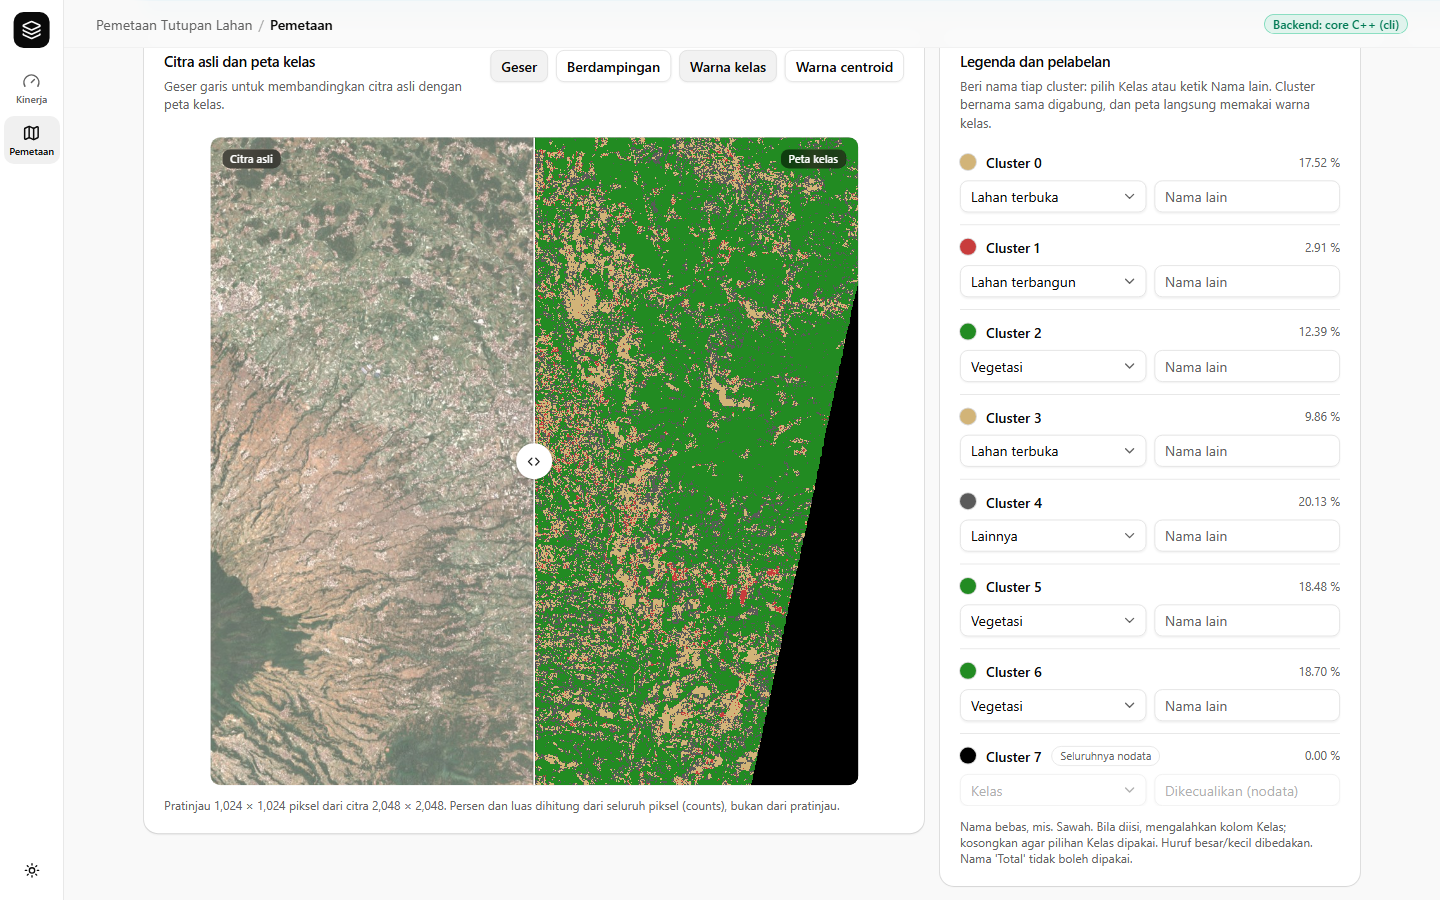
\includegraphics[width=0.95\textwidth]{ui_pemetaan_citra_vs_peta.png}
\caption{Halaman Pemetaan: citra asli dan peta kelas dengan penggeser sebelum/sesudah, serta legenda yang sekaligus menjadi panel pelabelan}
\label{fig:uipemetaan}
\end{figure}

\begin{figure}[H]
\centering
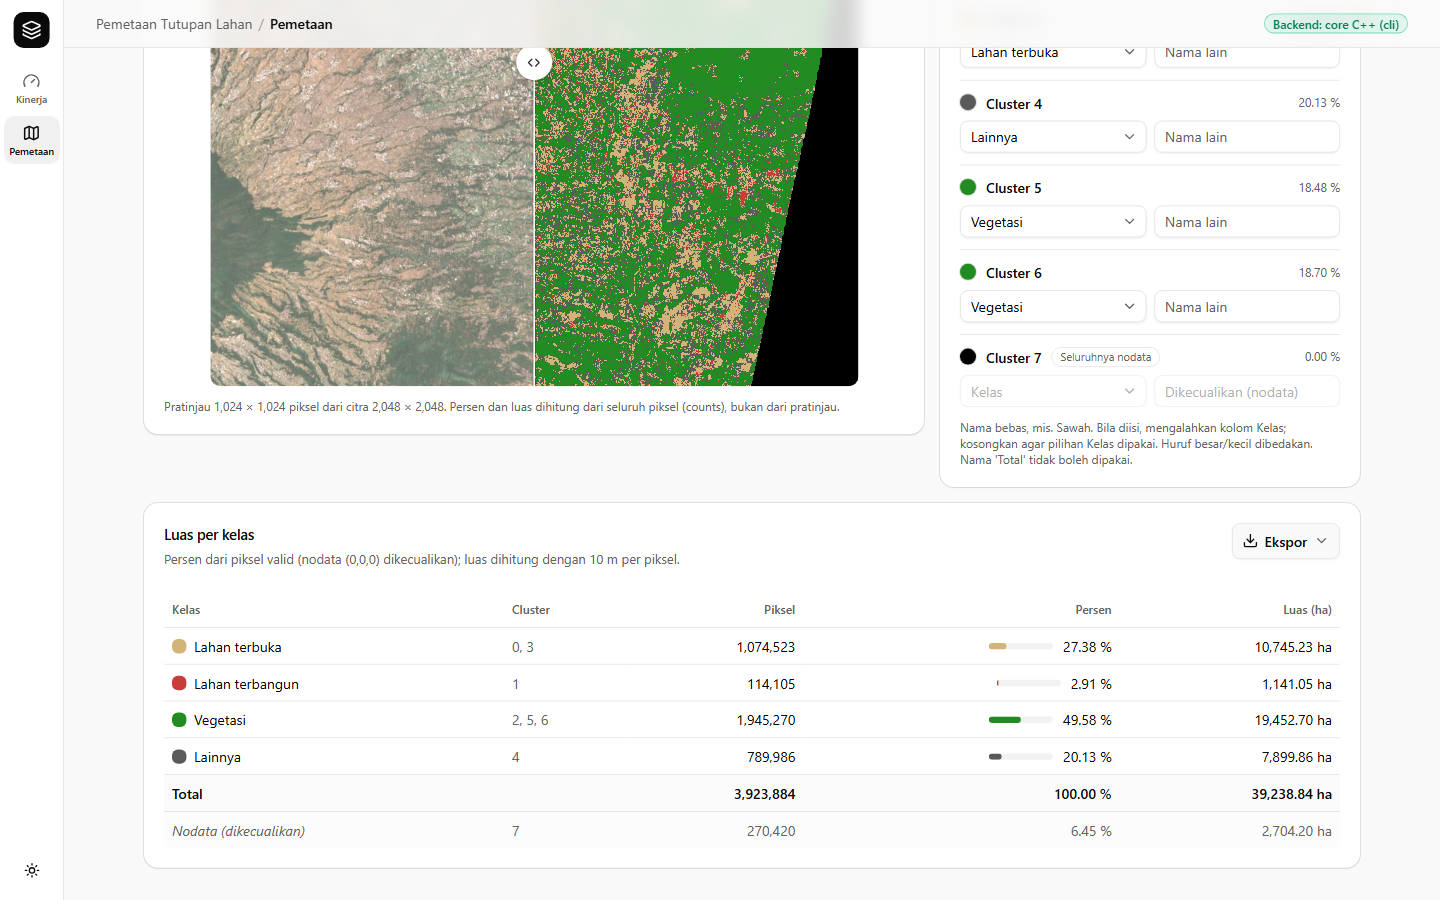
\includegraphics[width=0.95\textwidth]{ui_pemetaan_legenda_luas.png}
\caption{Halaman Pemetaan: tabel persentase dan luas per kelas, dengan baris \emph{nodata} yang dikecualikan dan menu ekspor}
\label{fig:uiluas}
\end{figure}

\begin{figure}[H]
\centering
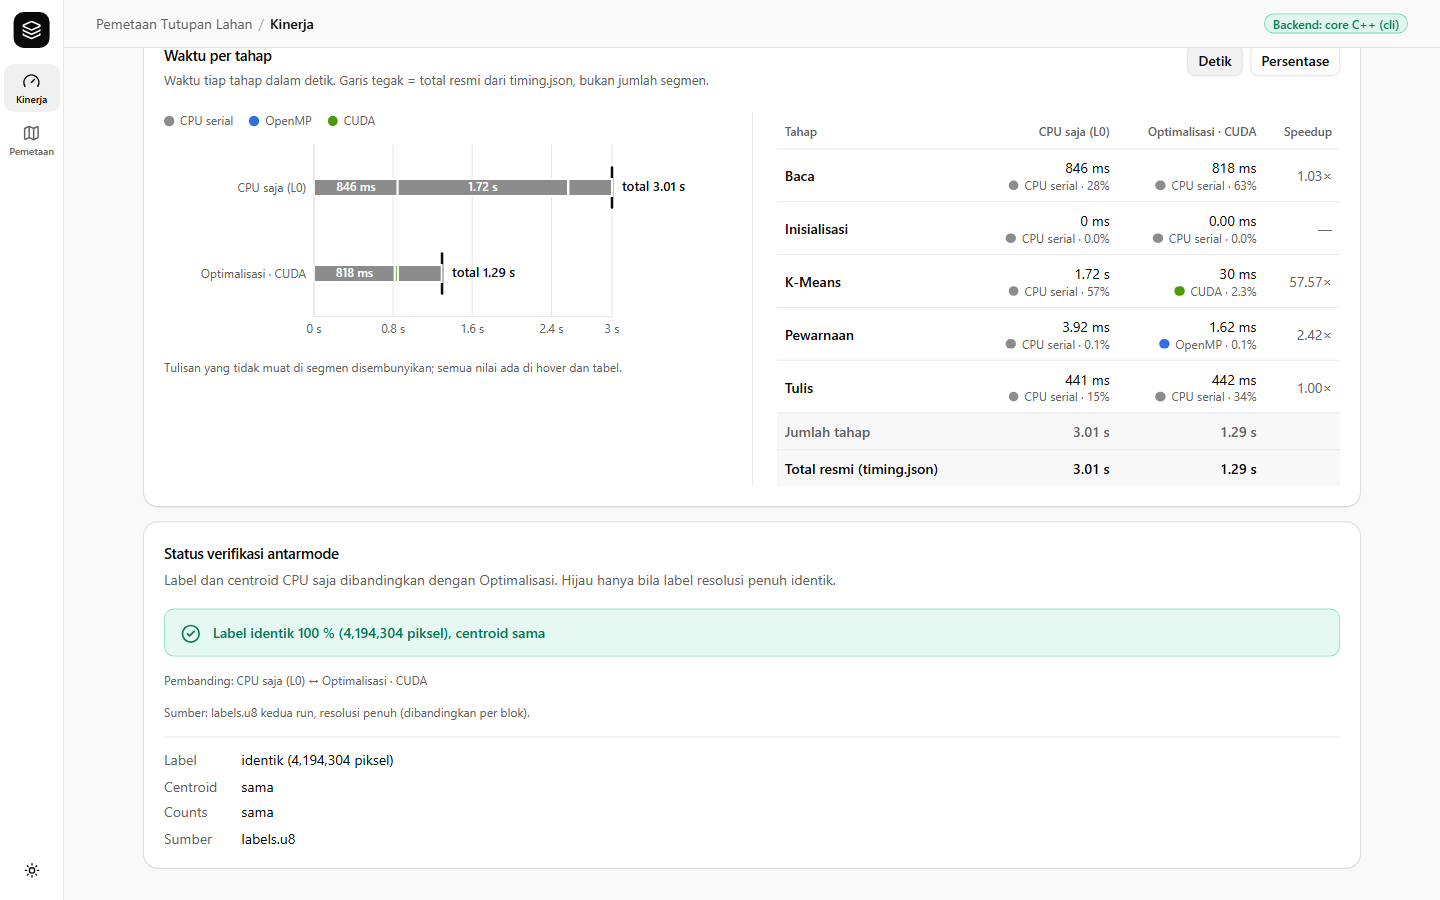
\includegraphics[width=0.95\textwidth]{ui_kinerja_tahap_verifikasi.png}
\caption[Halaman Kinerja: waktu per tahap beserta perangkatnya dan status verifikasi antarmode]{Halaman Kinerja: waktu per tahap beserta perangkatnya dan status verifikasi antarmode. Tangkapan layar ini hanya menunjukkan tata letak; angka di dalamnya berasal dari laptop uji fungsional dengan \emph{build} lama dan bukan hasil kinerja resmi (Bab~V). Pada \emph{build} itu \kode{kmeans\_omp} belum terhubung ke \kode{landcover}; pada \kode{main} OpenMP sudah terhubung dan mode otomatis memakai ambang $N\times K$}
\label{fig:uikinerja}
\end{figure}

\section{Pelabelan dan Perhitungan Luas}
\label{sec:pelabelan}
Setiap kelompok diberi nama kelas dari daftar pilihan (vegetasi, air, lahan terbangun, lahan terbuka, awan/bayangan, lainnya) atau nama bebas. Beberapa kelompok boleh diberi nama yang sama sehingga tergabung menjadi satu kelas, dan peta langsung diwarnai ulang menurut kelasnya. Nama kelas per \emph{run} disimpan di peramban dan dikirim ke API saat tabel luas diminta.

Semua angka luas berasal dari \kode{counts.json}, yaitu jumlah piksel bilangan bulat per kelompok dari label resolusi penuh, bukan dari pratinjau (\kode{app/landcover/labeling.py}). Piksel \emph{nodata} $(0,0,0)$ selalu jatuh ke satu kelompok yang sama; \kode{landcover} memeriksa hal ini, dan jumlahnya dikurangkan dari kelompok tersebut. Untuk kelas $k$ yang terdiri atas himpunan kelompok $C_k$, dengan $n_j$ jumlah piksel kelompok $j$, $N$ jumlah piksel citra, $N_{\text{nodata}}$ jumlah piksel \emph{nodata}, dan $s$ ukuran piksel dalam meter,
\begin{equation}
    \text{persen}_k = \frac{100 \sum_{j \in C_k} n'_j}{N - N_{\text{nodata}}}, \qquad
    \text{luas}_k = \frac{s^2 \sum_{j \in C_k} n'_j}{10\,000}\ \text{ha},
    \label{eq:luas}
\end{equation}
dengan $n'_j$ jumlah piksel kelompok $j$ setelah piksel \emph{nodata} dikurangkan. Untuk resolusi 10 meter, satu piksel sama dengan 0,01~ha. Kelompok berjumlah nol piksel sah (misalnya bila $K$ lebih besar daripada jumlah warna unik) dan ditampilkan sebagai 0\%, tanpa pembagian dengan jumlah piksel kelompok. Hasil dapat diekspor sebagai PNG pratinjau, CSV luas per kelas, CSV per kelompok, dan PNG peta resolusi penuh yang dibuat dari \kode{labels.u8} (\kode{app/landcover/export.py}).

\section{Stack Teknologi}
\label{sec:stack}
\emph{Stack} teknologi yang dipakai ditunjukkan pada Tabel~\ref{tab:stack}. Dibandingkan usulan di proposal, ada tiga perubahan: antarmuka memakai web React dengan API FastAPI (Streamlit hanya tersisa sebagai cadangan), \emph{build} memakai Make (bukan CMake), dan penulisan PNG memakai penulis paralel buatan sendiri.

\begin{table}[H]
\centering
\caption{\emph{Stack} teknologi yang dipakai}
\label{tab:stack}
\begin{tabularx}{\textwidth}{|L{4cm}|Y|}
\hline
\hdr{Komponen} & \hdr{Pilihan} \\ \hline
Inti pemrosesan & C++17 dan OpenMP (GCC 13.3), CUDA C++ (\kode{nvcc} 12.9, \kode{-arch=sm\_86}), semuanya dengan \kode{-O3} \\ \hline
Baca/tulis citra & Baca dengan \kode{stb\_image}; tulis dengan penulis PNG paralel sendiri (\kode{src/cli/png\_io\_omp.cpp}, bawaan Makefile), \kode{stb\_image\_write} tetap tersedia sebagai cadangan \\ \hline
Persiapan data & GDAL (\kode{gdal\_translate}) untuk konversi dan pemotongan kanal Sentinel-2 menjadi PNG \\ \hline
Pengukuran & \emph{Timer} per tahap di dalam program dan CUDA \emph{events} \\ \hline
\emph{Build} & GNU Make di Linux (WSL 2) \\ \hline
Antarmuka & React, TypeScript, Vite, Tailwind CSS, shadcn/ui, Recharts, dan TanStack Query, dengan API FastAPI dan uvicorn (Python) \\ \hline
Analisis data & Python (skrip di \kode{bench/}) untuk tabel dan grafik \\ \hline
Pengujian & \kode{pytest} untuk aplikasi; program uji C++ untuk inti \\ \hline
\end{tabularx}
\end{table}

\section{Pengujian Perangkat Lunak}
\label{sec:pengujianpl}
Pengujian dilakukan di dua lapis.
\begin{itemize}
    \item \textbf{Inti (C++, WSL):} \kode{test\_ref} menguji referensi CPU; \kode{test\_cuda\_vs\_ref} membandingkan setiap varian CUDA dengan referensi pada banyak ukuran citra dan nilai $K$; \kode{test\_omp\_vs\_cpu} membandingkan \kode{kmeans\_omp} dengan \kode{kmeans\_cpu}; \kode{test\_png\_omp} memastikan PNG dari penulis paralel terdekode menjadi piksel yang sama persis dengan masukan untuk berbagai jumlah \emph{thread}. Semua dijalankan lewat target Make (\kode{make test}, \kode{make test-omp}, \kode{make test-png-omp}).
    \item \textbf{Aplikasi (Python):} \kode{pytest} menguji pembaca kontrak, pelabelan dan luas, ekspor, API, peluncur, dan logika tampilan, termasuk tes dengan program \kode{landcover} asli lewat pembungkus WSL.
\end{itemize}
Hasil pengujian ini dirangkum di Subbab~\ref{sec:hasilverifikasi}.

% bab4.tex - Metodologi dan Implementasi Optimasi.
% Sumber: src/cpu/kmeans_cpu.cpp, src/omp/kmeans_omp.cpp, src/cuda/kmeans_cuda.cu, src/cuda/kmeans_cuda_variants.h,
% src/common/{kmeans.h,init.cpp,verify.h}, src/cli/{landcover.cpp,png_io_omp.cpp}, Makefile, docs/AMBANG_AUTO.md.
% TANPA angka kinerja (semua hasil ukur ada di Bab V).
\chapter{METODOLOGI DAN IMPLEMENTASI OPTIMASI}

\section{Alur Optimasi Berbasis \emph{Bottleneck}}
\label{sec:alur}
Optimasi dilakukan secara bertahap mengikuti siklus ukur, optimasi, lalu ukur kembali:
\begin{enumerate}
    \item Menjalankan mode CPU saja dan mengukur waktu setiap tahap dengan \emph{timer} di dalam program.
    \item Menentukan tahap yang paling dominan sebagai \emph{bottleneck}.
    \item Mengoptimasi tahap tersebut dengan perangkat dan teknik yang paling sesuai.
    \item Mengukur kembali waktu \emph{end-to-end} dan waktu per tahap untuk membuktikan peningkatannya, lalu mengulang dari langkah kedua untuk \emph{bottleneck} berikutnya.
\end{enumerate}

Dalam pelaksanaannya, urutan langkah mengikuti rencana proposal yang didasarkan pada kompleksitas algoritma, karena setiap modul dikerjakan oleh anggota yang berbeda secara bersamaan. K-Means dipindahkan ke GPU (L1), termasuk varian dengan \emph{streams} dan \emph{pinned memory} (L3). K-Means dan tahap pendukung (pewarnaan, \emph{counts}, dan tulis PNG) diparalelkan dengan OpenMP (L2). Keduanya lalu digabung di \kode{landcover}: K-Means di GPU dan tahap pendukung dengan OpenMP (L1+L2). \emph{Profiling} L0 yang dijalankan kemudian memastikan bahwa K-Means memang tahap terberat (Subbab~\ref{sec:profil}), dan pengukuran ulang setelah L1+L2 menunjukkan \emph{bottleneck} berikutnya. Konfigurasi setiap langkah ditunjukkan pada Tabel~\ref{tab:langkah}; hasil ukurnya ada di Subbab~\ref{sec:bertahap}.

\begin{table}[H]
\centering
\caption{Langkah optimasi yang diukur}
\label{tab:langkah}
\begin{tabularx}{\textwidth}{|L{2cm}|Y|}
\hline
\hdr{Langkah} & \hdr{Konfigurasi} \\ \hline
L0 & Mode CPU saja: semua tahap serial, K-Means dengan \kode{kmeans\_cpu} \\ \hline
L1 & K-Means di GPU (\kode{kmeans\_cuda}), tahap lain serial \\ \hline
L2 & K-Means dengan OpenMP (\kode{kmeans\_omp}) dan tahap pendukung dengan OpenMP, untuk 1--16 \emph{thread} \\ \hline
L1+L2 & K-Means di GPU dan tahap pendukung dengan OpenMP; ini konfigurasi mode Optimalisasi untuk pekerjaan besar \\ \hline
L3 & Varian \kode{kmeans\_cuda\_streams}: transfer per potongan lewat \emph{pinned memory} dan dua \emph{stream} (Subbab~\ref{sec:bersamaan}) \\ \hline
\end{tabularx}
\end{table}

Proposal juga merencanakan \kode{perf} atau \kode{gprof} dan Nsight Systems. Pada pelaksanaannya \emph{profiling} cukup memakai \emph{timer} per tahap di dalam program dan CUDA \emph{events}, karena \kode{nsys} dan \kode{ncu} tidak terpasang di mesin uji.

\section{Mode CPU Saja (\emph{Baseline})}
\label{sec:l0}
K-Means L0 (\kode{src/cpu/kmeans\_cpu.cpp}) ditulis dalam C++ dan dikompilasi dengan \kode{-O3}, agar perbandingan terhadap mode Optimalisasi jujur. Pada mode CPU saja, \kode{landcover} menetapkan satu \emph{thread} OpenMP untuk seluruh proses, sehingga pewarnaan, \emph{counts}, dan penulis PNG menjalankan kode yang sama dengan mode Optimalisasi tetapi tanpa paralelisme. Selisih waktu antara kedua mode dengan demikian berasal dari paralelisasi, bukan dari perbedaan algoritma atau pustaka.

\section{Penempatan Tahap}
\label{sec:penempatan}
Penempatan akhir setiap tahap pada mode Optimalisasi ditunjukkan pada Tabel~\ref{tab:penempatan}. Penempatan ini mengikuti hasil \emph{profiling} dan diterapkan di \kode{src/cli/landcover.cpp} dan \kode{src/cli/png\_io\_omp.cpp}.

\begin{table}[H]
\centering
\caption{Penempatan tahap pada mode Optimalisasi}
\label{tab:penempatan}
\begin{tabularx}{\textwidth}{|L{3.2cm}|L{3.6cm}|Y|}
\hline
\hdr{Tahap} & \hdr{Perangkat} & \hdr{Alasan} \\ \hline
Baca dan dekode PNG & CPU serial (\kode{stb\_image}) & Satu aliran \emph{deflate} tidak bisa dipecah. Masukan berupa folder potongan PNG dengan \emph{manifest} dibaca paralel per potongan, tetapi tidak dipakai pada \emph{benchmark} \\ \hline
Inisialisasi \emph{centroid} & CPU serial & Pekerjaan sangat kecil, dan harus sama persis di semua mode \\ \hline
K-Means & CUDA bila $N \times K \geq 70$ juta, selain itu OpenMP & Komputasi terberat dan paralel per piksel; untuk pekerjaan kecil biaya GPU tidak sebanding (Subbab~\ref{sec:otomatis}) \\ \hline
\emph{Counts} dan \emph{nodata} & OpenMP & Paralel per piksel; pekerjaan pendamping di luar waktu total \\ \hline
Pratinjau dan \kode{labels.u8} & CPU serial & Pekerjaan pendamping antarmuka; pratinjau hanya mengambil sampel piksel \\ \hline
Pewarnaan peta & OpenMP & Ringan dan paralel per piksel \\ \hline
Tulis peta PNG & OpenMP per \emph{strip} & Pemampatan adalah bagian terberat penulisan dan dapat dipecah per \emph{strip} \\ \hline
\end{tabularx}
\end{table}

\section{K-Means di GPU (L1)}
\label{sec:cuda}
Implementasi CUDA ada di \kode{src/cuda/kmeans\_cuda.cu} dan dibuat dalam dua tahap dengan hasil identik:
\begin{itemize}
    \item \textbf{T3, \kode{kmeans\_cuda\_simple}}: setiap \emph{thread} menambahkan pikselnya ke akumulator jumlah dan hitungan 64-bit di memori global dengan \kode{atomicAdd}. Karena jutaan \emph{thread} menulis ke paling banyak $4K$ alamat yang sama, operasi \emph{atomic} global saling antre. Varian ini dipertahankan sebagai pembanding dan cadangan.
    \item \textbf{T4, \kode{kmeans\_cuda}} (versi utama, dipakai \kode{landcover}): setiap \emph{block} mengakumulasi di \emph{shared memory} dengan bilangan bulat 32-bit, lalu menggabungkan hasilnya ke akumulator global 64-bit sekali per \emph{block}. Jumlah piksel per \emph{block} dibatasi agar jumlah 32-bit per kanal tidak meluap.
\end{itemize}

Kedua varian memakai alur yang sama. \emph{Host} memvalidasi argumen, menghitung \emph{centroid} awal dengan fungsi bersama, lalu menyalin citra dan \emph{centroid} ke GPU satu kali. Seluruh iterasi kemudian berjalan di GPU: mengosongkan akumulator, menjalankan \emph{kernel} \emph{assignment} dan akumulasi, lalu \emph{kernel} \kode{update\_centroids}. \emph{Kernel} memakai 256 \emph{thread} per \emph{block} dengan \emph{grid-stride loop}, dan setiap \emph{block} memuat $K$ \emph{centroid} ke \emph{shared memory} karena jumlahnya kecil dan dibaca semua \emph{thread}. Karena \emph{update} juga berjalan di GPU, tidak ada data yang berpindah antara CPU dan GPU di antara iterasi; label dan \emph{centroid} disalin kembali satu kali di akhir. Piksel disimpan sebagai \kode{uint8} (3 \emph{byte} per piksel), sedangkan label disimpan sebagai \kode{int32} sesuai antarmuka bersama.

Waktu salin ke GPU (h2d), seluruh \emph{loop} iterasi (\emph{kernel}), dan salin kembali (d2h) diukur dengan CUDA \emph{events}. Inisialisasi konteks CUDA tidak masuk ke waktu K-Means maupun waktu total karena \kode{landcover} melakukan pemanasan lebih dulu (Subbab~\ref{sec:kontrak}).

\section{K-Means dan Tahap Pendukung dengan OpenMP (L2)}
\label{sec:omp}
\begin{itemize}
    \item \textbf{K-Means} (\kode{src/omp/kmeans\_omp.cpp}): setiap iterasi membuka satu daerah paralel. \emph{Loop} piksel dibagi dengan \kode{\#pragma omp for schedule(static) nowait}. Setiap \emph{thread} memakai \emph{array} jumlah dan hitungan 64-bit miliknya sendiri di \emph{stack}, lalu menggabungkannya ke \emph{array} bersama di bagian \kode{critical} setelah \emph{loop}. Dengan cara ini tidak ada \kode{atomic} atau \kode{critical} di dalam \emph{loop} piksel. \emph{Update centroid} yang hanya $K$ elemen tetap serial.
    \item \textbf{\emph{Counts} dan \emph{nodata}}: pola yang sama, yaitu hitungan lokal per \emph{thread} yang digabung di bagian \kode{critical}.
    \item \textbf{Pewarnaan peta}: \kode{\#pragma omp parallel for schedule(static)} yang mengganti label setiap piksel dengan warna \emph{centroid}-nya, langsung di atas \emph{buffer} citra.
    \item \textbf{Tulis PNG} (\kode{src/cli/png\_io\_omp.cpp}): penulis PNG buatan sendiri bergaya \kode{pigz}. Citra dibagi menjadi \emph{strip} baris berukuran tetap; setiap \emph{strip} difilter, dimampatkan (LZ77 dengan kode Huffman tetap), dan dihitung \emph{checksum}-nya oleh satu \emph{thread}, lalu \emph{strip} disambung berurutan. Karena setiap \emph{strip} dimampatkan mandiri, berkas keluaran identik \emph{byte} demi \emph{byte} untuk berapa pun jumlah \emph{thread}, dan piksel hasil dekodenya sama persis dengan masukan.
\end{itemize}

\section{Kerja Bersamaan CPU dan GPU (L3)}
\label{sec:bersamaan}
Yang dibuat untuk langkah ini adalah varian \kode{kmeans\_cuda\_streams}, yang dideklarasikan di \kode{src/cuda/\allowbreak kmeans\_cuda\_variants.h}. \emph{Kernel}-nya sama dengan T4, tetapi citra dikirim dan label diambil per potongan lewat \emph{pinned memory} dan dua CUDA \emph{stream}, sehingga transfer tumpang tindih dengan \emph{assignment} pada iterasi pertama dan terakhir. Hasilnya identik dengan \kode{kmeans\_cuda}.

Rencana di proposal belum seluruhnya terlaksana. Varian ini hanya diukur di tingkat \emph{kernel} (program \kode{tests/bench\_cuda}) dan tidak dipanggil oleh \kode{landcover}, sehingga tidak ada di \emph{pipeline} maupun aplikasi. \emph{Pipeline} beberapa wilayah, yaitu GPU menjalankan K-Means wilayah ke-$i$ sementara CPU membaca wilayah ke-$(i+1)$ dan menulis wilayah ke-$(i-1)$, juga belum dibuat. Hasil ukur varian ini dibahas di Subbab~\ref{sec:hasilcuda}.

\section{Pemilihan Mode Otomatis}
\label{sec:otomatis}
Pada mode Optimalisasi dengan \kode{-{}-kmeans auto}, \kode{landcover} memilih CUDA bila
\begin{equation}
    N \times K \geq 70 \text{ juta},
    \label{eq:ambang}
\end{equation}
dan OpenMP bila tidak, dengan $N$ jumlah piksel dan $K$ jumlah kelompok. Bila CUDA tidak terhubung pada \emph{build}, pilihan jatuh ke OpenMP, lalu ke serial. Bila \kode{kmeans\_cuda} gagal saat berjalan, K-Means diulang dengan OpenMP (atau serial bila OpenMP tidak terhubung). Alasan pemilihan dicatat di \kode{meta.json} dan ditampilkan di antarmuka.

Ambang ini berubah dua kali. Ambang awal sebesar 8 juta piksel hanya perkiraan sementara sebelum ada data. Ambang kedua, 100 ribu piksel, diturunkan dari waktu total yang tidak memuat pemanasan CUDA. Ambang ketiga, yang dipakai sekarang (Persamaan~\ref{eq:ambang}), diturunkan dari waktu dinding seluruh proses dengan dua alasan:
\begin{enumerate}
    \item Waktu K-Means OpenMP tumbuh sebanding dengan $N \times K$, sedangkan waktu K-Means CUDA hampir tidak bergantung pada $K$. Karena itu titik impasnya bergantung pada $N \times K$, bukan pada $N$ saja.
    \item Setiap \emph{run} dari antarmuka menjalankan proses \kode{landcover} baru, sehingga inisialisasi konteks CUDA selalu dirasakan pengguna walaupun tidak masuk waktu total.
\end{enumerate}
Penurunan ambang ini dapat diulang dengan \kode{bench/fit\_auto\_threshold.py}; datanya dibahas di Subbab~\ref{sec:hasilambang}.

\section{Jaminan Konsistensi Hasil}
\label{sec:konsistensi}
Agar semua mode menghasilkan keluaran identik, seluruh perhitungan inti memakai aritmetika bilangan bulat dengan aturan yang sama di \kode{kmeans\_cpu}, \kode{kmeans\_omp}, dan \kode{kmeans\_cuda}:
\begin{itemize}
    \item \textbf{Jarak}: kuadrat selisih R, G, B antara piksel dan \emph{centroid} dihitung dalam \kode{int32}, sehingga hasilnya eksak.
    \item \textbf{Penjumlahan}: jumlah warna dan hitungan per kelompok diakumulasi dalam bilangan bulat 64-bit tak bertanda, sehingga hasilnya tidak bergantung pada urutan penjumlahan.
    \item \textbf{\emph{Centroid} baru}: dihitung dengan pembagian bilangan bulat yang \textbf{dibulatkan ke bawah} untuk setiap kanal $c$ (proposal menulis ``dibulatkan''; yang diterapkan adalah pembulatan ke bawah):
    \begin{equation}
        \mu_{j,c} = \left\lfloor \frac{\sum_{x_i \in S_j} x_{i,c}}{|S_j|} \right\rfloor .
        \label{eq:floor}
    \end{equation}
    \item \textbf{Jarak sama besar}: dipilih \emph{centroid} dengan indeks terkecil (perbandingan ``lebih kecil'' yang ketat).
    \item \textbf{\emph{Cluster} kosong}: \emph{centroid} lama dipertahankan.
    \item \textbf{\emph{Centroid} awal}: dipilih di CPU oleh satu fungsi bersama, \kode{kmeans\_init\_centroids} (\kode{src/common/init.cpp}), dengan pembangkit bilangan acak \emph{splitmix64} buatan sendiri dan \emph{seed} tetap. Setiap implementasi memanggil fungsi ini, sehingga \emph{centroid} awalnya sama.
    \item \textbf{Iterasi}: tepat sebanyak jumlah iterasi yang diminta, tanpa berhenti lebih awal.
\end{itemize}

Hasil diverifikasi di dua tempat. Program uji inti memakai \kode{verify\_identical} (\kode{src/common/verify.h}) yang menghitung jumlah label dan \emph{centroid} yang berbeda; target verifikasi adalah nol perbedaan. Aplikasi membandingkan \kode{labels.u8} resolusi penuh, \emph{centroid}, dan \emph{counts} antara \emph{run} mode CPU saja dan mode Optimalisasi (\kode{app/landcover/verify.py}). Status hijau ``Label identik 100\%'' hanya diberikan bila label resolusi penuh benar-benar sama; perbandingan yang hanya memakai pratinjau ditandai sebagai verifikasi parsial. Karena labelnya identik, persentase dan luas setiap kelas juga identik.

% bab5.tex - Hasil dan Pembahasan (Sesi B, L4-L5).
% Aturan: semua angka kinerja berasal dari tabel/*.tex dan makro tabel/angka.tex yang dibuat
% skrip/tabel_ke_tex.py dari bench/results/*.csv; JANGAN mengetik angka kinerja di berkas ini.
% Satu tabel satu mesin; data sintetis selalu ditandai; total_ms tanpa pemanasan CUDA, Proses dengan pemanasan.
\chapter{HASIL DAN PEMBAHASAN}

\section{Lingkungan dan Data Uji}
\label{sec:lingkungan}
Pengukuran dilakukan di tiga komputer anggota kelompok (Tabel~\ref{tab:mesin}). Agar angka tidak tercampur, setiap tabel di bab ini hanya memuat hasil dari satu mesin. Seluruh angka kinerja utama berasal dari Mesin B. Mesin A hanya dipakai untuk profil L0 sebagai pembanding, sedangkan Mesin C dipakai untuk uji fungsional aplikasi dengan citra Sentinel-2.

\begin{table}[H]
\centering
\caption{Mesin uji dan eksperimen yang dijalankan di masing-masing mesin}
\label{tab:mesin}
\small
\begin{tabularx}{\textwidth}{L{1.6cm}YY}
\hline
\hdr{Mesin} & \hdr{Spesifikasi} & \hdr{Eksperimen} \\ \hline
A & Intel Core i7-1065G7 (4 inti, 8 \emph{thread}), RAM 16 GB; WSL 2, GCC 11.4 & Profil L0 (Tabel~\ref{tab:l0a}), hanya sebagai pembanding \\ \hline
B & Intel Core i7-13620H (16 CPU logis di WSL), NVIDIA RTX 3050 6 GB Laptop (\kode{sm\_86}, \emph{driver} 576.93), RAM WSL 7,6 GiB; WSL 2 Ubuntu 24.04, CUDA 12.9, GCC 13.3; skema daya \emph{Balanced} & Semua \emph{benchmark} kinerja: per tahap, optimasi bertahap, \emph{strong}/\emph{weak scaling}, varian CUDA, ambang mode otomatis \\ \hline
C & Intel Core i7-13650HX, NVIDIA RTX 3050 6 GB Laptop; WSL 2 Ubuntu 24.04 & Uji fungsional Sentinel-2, verifikasi \kode{cmp}, tangkapan layar aplikasi. Waktunya bukan hasil kinerja resmi \\ \hline
\end{tabularx}
\par\smallskip\footnotesize\raggedright Sumber: \kode{bench/results/run\_20261127\_1634\_env.txt} dan \kode{bench/BENCH\_GPU.md} (B), \kode{docs/PROFIL\_L0.md} (A), \kode{meta.json} \emph{run} Sentinel-2 (C).
\end{table}

\textbf{Data uji.} Ada dua jenis citra:
\begin{itemize}
    \item \textbf{Citra sintetis} (\kode{sintetis\_lanskap\_\textless lebar\textgreater x\textless tinggi\textgreater}) yang dibangkitkan skrip \emph{benchmark}, berukuran 1000$\times$1000, 2000$\times$2000, 4000$\times$3000, dan 7680$\times$4320 piksel untuk pengukuran utama; 320$\times$320 sampai 4000$\times$3000 untuk penentuan ambang; dan 2000$\times$1000 sampai 32000$\times$1000 untuk \emph{weak scaling}. Varian CUDA diukur pada citra acak. \textbf{Semua angka kinerja di Subbab~\ref{sec:profil} sampai~\ref{sec:hasilambang} berasal dari citra sintetis.}
    \item \textbf{Citra Sentinel-2} \emph{tile} T49MDM (\kode{S2B\_MSIL2A\_20261017}), kanal B04/B03/B02, berupa potongan 512, 1024, dan 2048 piksel persegi. Citra ini dipakai untuk uji fungsional dan verifikasi (Subbab~\ref{sec:hasilverifikasi} dan~\ref{sec:hasilsentinel}).
\end{itemize}

\textbf{Prosedur.} Setiap konfigurasi dijalankan satu kali sebagai pemanasan (dibuang), lalu lima kali; yang dilaporkan adalah median. Semua \emph{run} memakai 20 iterasi dan \emph{seed} 42. Waktu diambil dari \kode{timing.json} keluaran \kode{landcover} (Subbab~\ref{sec:kontrak}). \textbf{Total} adalah \kode{total\_ms}, yaitu baca + K-Means + pewarnaan + tulis, tanpa pemanasan konteks CUDA. \textbf{Proses} adalah waktu dinding satu proses \kode{landcover} (\kode{wall\_ms}) yang mencakup pemanasan itu. Keduanya disajikan karena aplikasi menjalankan \kode{landcover} sebagai proses baru di setiap \emph{run}, sehingga pengguna merasakan Proses, bukan Total. Pada sesi Mesin B yang merekamnya (\emph{run} 16:34 dan sesi ambang), pemanasan konteks CUDA berkisar \WarmMin--\WarmMax~ms per proses.

\textbf{Penyimpangan dari rencana proposal.}
\begin{enumerate}
    \item Median dari 5 ulangan, bukan minimal 10.
    \item Ukuran citra 1000$^2$, 2000$^2$, 4000$\times$3000, dan 7680$\times$4320, bukan 2048$^2$, 4096$^2$, 8192$^2$, dan satu \emph{tile} penuh. \emph{Tile} penuh 10980$\times$10980 tidak tersedia (Subbab~\ref{sec:batasan}).
    \item \emph{Profiling} memakai pengukur waktu per tahap di dalam program dan CUDA \emph{events}, bukan \kode{perf}/\kode{gprof}; Nsight (\kode{nsys}/\kode{ncu}) tidak terpasang di mesin uji.
    \item Mesin uji adalah laptop anggota kelompok (Tabel~\ref{tab:mesin}), bukan mesin pada rencana proposal.
    \item Tahap baca PNG tetap serial di semua mode (Tabel~\ref{tab:penempatan}).
\end{enumerate}

\section{Profiling L0 dan \emph{Bottleneck}}
\label{sec:profil}
Tabel~\ref{tab:l0b} menunjukkan waktu setiap tahap pada mode CPU saja (L0, \kode{kmeans\_cpu} satu \emph{thread}) di Mesin B. Pada semua ukuran dan nilai $K$ yang diukur, K-Means adalah tahap terbesar dengan porsi \PorsiKMLoMin--\PorsiKMLoMax{} dari Total. Porsinya membesar seiring $K$, karena biaya \emph{assignment} sebanding dengan $N\times K$, sedangkan baca dan tulis PNG hanya bergantung pada jumlah piksel dan isi citra. Tahap inisialisasi praktis nol karena hanya memilih $K$ \emph{centroid} awal.

% DIBUAT OLEH laporan/skrip/tabel_ke_tex.py -- jangan disunting tangan.
\begin{table}[H]
\centering
\caption{Waktu per tahap mode CPU saja (L0) dan porsi K-Means, citra sintetis, Mesin B (ms)}
\label{tab:l0b}
\small
\begin{tabularx}{\textwidth}{L{2.3cm}r>{\raggedleft\arraybackslash}X>{\raggedleft\arraybackslash}X>{\raggedleft\arraybackslash}X>{\raggedleft\arraybackslash}X>{\raggedleft\arraybackslash}X>{\raggedleft\arraybackslash}X>{\raggedleft\arraybackslash}X}
\hline
\hdr{Citra} & \hdr{$K$} & \hdr{Baca} & \hdr{Init} & \hdr{K-Means} & \hdr{Warna} & \hdr{Tulis} & \hdr{Total} & \hdr{Porsi K-Means} \\ \hline
4000$\times$3000 & 2 & 167,2 & 0,0 & 640,7 & 10,0 & 50,4 & 875,1 & 73\% \\ \hline
4000$\times$3000 & 4 & 156,1 & 0,0 & 1017,2 & 9,6 & 51,9 & 1224,8 & 83\% \\ \hline
1000$\times$1000 & 8 & 13,2 & 0,0 & 207,5 & 0,7 & 17,4 & 237,4 & 87\% \\ \hline
2000$\times$2000 & 8 & 52,9 & 0,0 & 777,4 & 4,0 & 85,8 & 921,7 & 84\% \\ \hline
4000$\times$3000 & 8 & 161,5 & 0,0 & 2385,1 & 11,8 & 215,2 & 2750,3 & 87\% \\ \hline
7680$\times$4320 & 8 & 431,3 & 0,0 & 5870,6 & 24,0 & 419,3 & 6765,7 & 87\% \\ \hline
4000$\times$3000 & 16 & 170,7 & 0,0 & 4794,6 & 13,8 & 417,7 & 5400,7 & 89\% \\ \hline
\end{tabularx}
\par\smallskip\footnotesize\raggedright Median 5 ulangan setelah 1 pemanasan, 20 iterasi, \emph{seed} 42. Sumber: \kode{bench\_gpu\_summary.csv} dan \kode{run\_20261127\_1634\_ksweep\_summary.csv} (4000$\times$3000 dari \emph{run} 16:34).
\end{table}


Pola yang sama muncul di Mesin A (Tabel~\ref{tab:l0a}): porsi K-Means \PorsiKMAMin--\PorsiKMAMax. Waktu mutlak kedua mesin berbeda dan tidak dibandingkan. Yang penting adalah kesimpulannya sama di dua mesin: K-Means adalah \emph{bottleneck} utama L0, sehingga menjadi sasaran pertama L1 (CUDA) dan L2 (OpenMP). Sesudah K-Means, tahap berikutnya yang terbesar adalah tulis dan baca PNG.

% DIBUAT OLEH laporan/skrip/tabel_ke_tex.py -- jangan disunting tangan.
\begin{table}[H]
\centering
\caption{Pembanding: waktu per tahap L0 di Mesin A (i7-1065G7), citra sintetis (ms)}
\label{tab:l0a}
\small
\begin{tabularx}{\textwidth}{L{2.3cm}r>{\raggedleft\arraybackslash}X>{\raggedleft\arraybackslash}X>{\raggedleft\arraybackslash}X>{\raggedleft\arraybackslash}X>{\raggedleft\arraybackslash}X>{\raggedleft\arraybackslash}X>{\raggedleft\arraybackslash}X}
\hline
\hdr{Citra} & \hdr{$K$} & \hdr{Baca} & \hdr{Init} & \hdr{K-Means} & \hdr{Warna} & \hdr{Tulis} & \hdr{Total} & \hdr{Porsi K-Means} \\ \hline
1000$\times$1000 & 8 & 19,0 & 0,0 & 313,9 & 0,9 & 42,8 & 375,1 & 84\% \\ \hline
2000$\times$2000 & 8 & 67,0 & 0,0 & 1038,5 & 3,3 & 214,0 & 1322,8 & 79\% \\ \hline
4000$\times$3000 & 8 & 201,0 & 0,0 & 3084,7 & 10,1 & 521,2 & 3827,2 & 81\% \\ \hline
7680$\times$4320 & 8 & 569,4 & 0,0 & 8483,4 & 29,1 & 1198,9 & 10263,9 & 83\% \\ \hline
4000$\times$3000 & 4 & 206,4 & 0,0 & 1514,7 & 9,9 & 267,4 & 2002,5 & 76\% \\ \hline
4000$\times$3000 & 16 & 208,6 & 0,0 & 6556,9 & 10,8 & 1073,6 & 7871,4 & 83\% \\ \hline
\end{tabularx}
\par\smallskip\footnotesize\raggedright Median 5 ulangan setelah 1 pemanasan. Sumber: \kode{docs/PROFIL\_L0\_tabel.md} (\kode{bench/profile\_l0.py}). Mesin berbeda dengan tabel lain di bab ini; angkanya tidak dibandingkan langsung dengan Mesin B.
\end{table}


\section{Optimasi Bertahap}
\label{sec:bertahap}
Tabel~\ref{tab:bertahapk8} membandingkan langkah optimasi pada $K=8$ untuk empat ukuran citra. Untuk L2 dan L1+L2, yang ditampilkan adalah jumlah \emph{thread} OpenMP dengan Total terkecil. Gambar~\ref{fig:tahap} menampilkan komposisi tahap pada citra terbesar.

% DIBUAT OLEH laporan/skrip/tabel_ke_tex.py -- jangan disunting tangan.
\begin{table}[H]
\centering
\caption{Optimasi bertahap L0 $\rightarrow$ L2 $\rightarrow$ L1 $\rightarrow$ L1+L2, $K=8$, citra sintetis, Mesin B (ms; $S$ = \emph{speedup} terhadap L0)}
\label{tab:bertahapk8}
\footnotesize
\begin{tabularx}{\textwidth}{L{2.1cm}rL{2.3cm}>{\raggedleft\arraybackslash}X>{\raggedleft\arraybackslash}X>{\raggedleft\arraybackslash}X>{\raggedleft\arraybackslash}X>{\raggedleft\arraybackslash}X>{\raggedleft\arraybackslash}X}
\hline
\hdr{Citra} & \hdr{$K$} & \hdr{Konfigurasi} & \hdr{K-Means} & \hdr{$S$ K-Means} & \hdr{Total} & \hdr{$S$ Total} & \hdr{Proses} & \hdr{$S$ Proses} \\ \hline
1000$\times$1000 & 8 & L0 & 207,5 & 1,0\ensuremath{\times} & 237,4 & 1,00\ensuremath{\times} & -- & -- \\ \hline
1000$\times$1000 & 8 & L2 (8 thr) & 43,5 & 4,8\ensuremath{\times} & 73,7 & 3,22\ensuremath{\times} & -- & -- \\ \hline
1000$\times$1000 & 8 & L1 & 4,8 & 42,9\ensuremath{\times} & 37,4 & 6,35\ensuremath{\times} & -- & -- \\ \hline
1000$\times$1000 & 8 & L1+L2 (2 thr) & 5,1 & 40,6\ensuremath{\times} & 34,5 & 6,89\ensuremath{\times} & -- & -- \\ \hline
2000$\times$2000 & 8 & L0 & 777,4 & 1,0\ensuremath{\times} & 921,7 & 1,00\ensuremath{\times} & -- & -- \\ \hline
2000$\times$2000 & 8 & L2 (8 thr) & 165,0 & 4,7\ensuremath{\times} & 245,1 & 3,76\ensuremath{\times} & -- & -- \\ \hline
2000$\times$2000 & 8 & L1 & 18,5 & 41,9\ensuremath{\times} & 159,5 & 5,78\ensuremath{\times} & -- & -- \\ \hline
2000$\times$2000 & 8 & L1+L2 (4 thr) & 17,9 & 43,4\ensuremath{\times} & 112,7 & 8,18\ensuremath{\times} & -- & -- \\ \hline
4000$\times$3000 & 8 & L0 & 2385,1 & 1,0\ensuremath{\times} & 2750,3 & 1,00\ensuremath{\times} & 2800,7 & 1,00\ensuremath{\times} \\ \hline
4000$\times$3000 & 8 & L2 (16 thr) & 337,3 & 7,1\ensuremath{\times} & 560,7 & 4,90\ensuremath{\times} & 617,2 & 4,54\ensuremath{\times} \\ \hline
4000$\times$3000 & 8 & L1 & 55,7 & 42,8\ensuremath{\times} & 436,2 & 6,31\ensuremath{\times} & 720,3 & 3,89\ensuremath{\times} \\ \hline
4000$\times$3000 & 8 & L1+L2 (8 thr) & 55,4 & 43,1\ensuremath{\times} & 291,9 & 9,42\ensuremath{\times} & 600,7 & 4,66\ensuremath{\times} \\ \hline
7680$\times$4320 & 8 & L0 & 5870,6 & 1,0\ensuremath{\times} & 6765,7 & 1,00\ensuremath{\times} & -- & -- \\ \hline
7680$\times$4320 & 8 & L2 (8 thr) & 1258,0 & 4,7\ensuremath{\times} & 1875,9 & 3,61\ensuremath{\times} & -- & -- \\ \hline
7680$\times$4320 & 8 & L1 & 138,9 & 42,3\ensuremath{\times} & 1033,1 & 6,55\ensuremath{\times} & -- & -- \\ \hline
7680$\times$4320 & 8 & L1+L2 (16 thr) & 131,8 & 44,6\ensuremath{\times} & 684,1 & 9,89\ensuremath{\times} & -- & -- \\ \hline
\end{tabularx}
\par\smallskip\footnotesize\raggedright L2 dan L1+L2: konfigurasi terbaik menurut Total; ``thr'' = jumlah \emph{thread} OpenMP. Total = \kode{total\_ms}, tanpa pemanasan konteks CUDA. Proses = waktu dinding satu proses \kode{landcover} (\kode{wall\_ms}), termasuk pemanasan. ``--'' = tidak diukur: sesi \kode{bench\_gpu} (1000$^2$, 2000$^2$, 7680$\times$4320) belum merekam \kode{wall\_ms}; baris 4000$\times$3000 dari \emph{run} 16:34.
\end{table}


\begin{figure}[H]
\centering
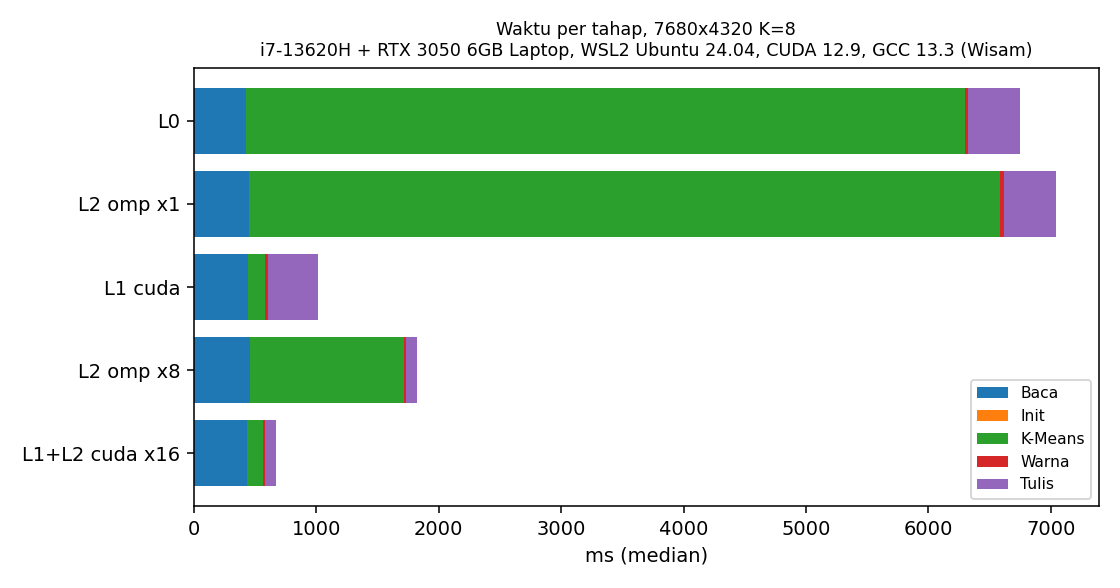
\includegraphics[width=0.92\textwidth]{tahap_7680x4320_k8.png}
\caption{Waktu per tahap pada citra sintetis 7680$\times$4320, $K=8$, Mesin B (median, ms). Sumber: \kode{docs/fig/mesinWisam/}, dibuat \kode{bench/analyze\_scaling.py}}
\label{fig:tahap}
\end{figure}

Pada 7680$\times$4320 dengan $K=8$, Total turun dari \LoTotalDelapan~ms (L0) menjadi \LdLdTotalDelapan~ms pada L1+L2 (\LdLdCfgDelapan), atau \LdLdSTotalDelapan. Kontribusi setiap langkah adalah sebagai berikut:
\begin{itemize}
    \item \textbf{L1 (CUDA).} K-Means turun dari \LoKMDelapan{} menjadi \LdKMDelapan~ms (\LdSKMDelapan), tetapi Total hanya membaik \LdSTotalDelapan. Penyebabnya, waktu di luar K-Means (Total dikurangi K-Means) hampir tidak berubah: \LuarLoDelapan~ms pada L0 dan \LuarLdDelapan~ms pada L1.
    \item \textbf{L2 (OpenMP).} Sendirian, L2 (\LdbCfgDelapan) memberi \LdbSTotalDelapan{} pada Total. Kontribusi terbesarnya justru pada kombinasi dengan L1, karena L2 juga memparalelkan pewarnaan dan tulis PNG.
    \item \textbf{L1+L2.} Waktu di luar K-Means turun menjadi \LuarLdLdDelapan~ms; tulis PNG saja turun dari \TulisLoDelapan{} menjadi \TulisLdLdDelapan~ms. Sisanya didominasi baca PNG (\BacaLdLdDelapan~ms, \PorsiBacaLdLdDelapan{} dari Total), yang tetap serial.
\end{itemize}

% DIBUAT OLEH laporan/skrip/tabel_ke_tex.py -- jangan disunting tangan.
\begin{table}[H]
\centering
\caption{Optimasi bertahap pada 4000$\times$3000 untuk $K=2$, 4, dan 16, citra sintetis, Mesin B (ms; $S$ = \emph{speedup} terhadap L0)}
\label{tab:bertahapk}
\footnotesize
\begin{tabularx}{\textwidth}{L{2.1cm}rL{2.3cm}>{\raggedleft\arraybackslash}X>{\raggedleft\arraybackslash}X>{\raggedleft\arraybackslash}X>{\raggedleft\arraybackslash}X>{\raggedleft\arraybackslash}X>{\raggedleft\arraybackslash}X}
\hline
\hdr{Citra} & \hdr{$K$} & \hdr{Konfigurasi} & \hdr{K-Means} & \hdr{$S$ K-Means} & \hdr{Total} & \hdr{$S$ Total} & \hdr{Proses} & \hdr{$S$ Proses} \\ \hline
4000$\times$3000 & 2 & L0 & 640,7 & 1,0\ensuremath{\times} & 875,1 & 1,00\ensuremath{\times} & 916,1 & 1,00\ensuremath{\times} \\ \hline
4000$\times$3000 & 2 & L2 (8 thr) & 197,0 & 3,3\ensuremath{\times} & 379,5 & 2,31\ensuremath{\times} & 415,5 & 2,20\ensuremath{\times} \\ \hline
4000$\times$3000 & 2 & L1 & 57,4 & 11,2\ensuremath{\times} & 275,5 & 3,18\ensuremath{\times} & 574,3 & 1,60\ensuremath{\times} \\ \hline
4000$\times$3000 & 2 & L1+L2 (4 thr) & 56,3 & 11,4\ensuremath{\times} & 248,7 & 3,52\ensuremath{\times} & 591,0 & 1,55\ensuremath{\times} \\ \hline
4000$\times$3000 & 4 & L0 & 1017,2 & 1,0\ensuremath{\times} & 1224,8 & 1,00\ensuremath{\times} & 1258,4 & 1,00\ensuremath{\times} \\ \hline
4000$\times$3000 & 4 & L2 (4 thr) & 302,2 & 3,4\ensuremath{\times} & 490,1 & 2,50\ensuremath{\times} & 516,0 & 2,44\ensuremath{\times} \\ \hline
4000$\times$3000 & 4 & L1 & 59,6 & 17,1\ensuremath{\times} & 314,6 & 3,89\ensuremath{\times} & 642,0 & 1,96\ensuremath{\times} \\ \hline
4000$\times$3000 & 4 & L1+L2 (2 thr) & 56,3 & 18,1\ensuremath{\times} & 249,1 & 4,92\ensuremath{\times} & 466,1 & 2,70\ensuremath{\times} \\ \hline
4000$\times$3000 & 16 & L0 & 4794,6 & 1,0\ensuremath{\times} & 5400,7 & 1,00\ensuremath{\times} & 5509,7 & 1,00\ensuremath{\times} \\ \hline
4000$\times$3000 & 16 & L2 (16 thr) & 684,2 & 7,0\ensuremath{\times} & 927,9 & 5,82\ensuremath{\times} & 1000,7 & 5,51\ensuremath{\times} \\ \hline
4000$\times$3000 & 16 & L1 & 59,7 & 80,3\ensuremath{\times} & 609,9 & 8,86\ensuremath{\times} & 890,2 & 6,19\ensuremath{\times} \\ \hline
4000$\times$3000 & 16 & L1+L2 (16 thr) & 50,5 & 95,0\ensuremath{\times} & 300,6 & 17,97\ensuremath{\times} & 613,4 & 8,98\ensuremath{\times} \\ \hline
\end{tabularx}
\par\smallskip\footnotesize\raggedright Keterangan kolom sama dengan Tabel~\ref{tab:bertahapk8}. Sumber: \kode{run\_20261127\_1634\_ksweep\_summary.csv}.
\end{table}


\textbf{Total dan Proses.} Tabel~\ref{tab:bertahapk} memuat empat nilai $K$ pada 4000$\times$3000, satu-satunya ukuran yang Prosesnya terekam. Menurut Total, L1+L2 selalu paling cepat. Menurut Proses, pemanasan konteks CUDA menutup sebagian besar keuntungan GPU. Pada $K=8$, L1+L2 (\LdLdCfgEmpat) memberi \LdLdSTotalEmpat{} menurut Total tetapi hanya \LdLdSProsesEmpat{} menurut Proses. Konfigurasi Optimalisasi tercepat menurut Proses memberi \emph{speedup} \SProsesTerbaikKDua{} ($K=2$, \CfgProsesTerbaikKDua), \SProsesTerbaikKEmpat{} ($K=4$, \CfgProsesTerbaikKEmpat), \SProsesTerbaikKDelapan{} ($K=8$, \CfgProsesTerbaikKDelapan), dan \SProsesTerbaikKEnambelas{} ($K=16$, \CfgProsesTerbaikKEnambelas). Pada $K=2$, OpenMP tanpa GPU bahkan menjadi pilihan tercepat menurut Proses. Inilah dasar pemilihan mode otomatis (Subbab~\ref{sec:hasilambang}).

\section{\emph{Strong} dan \emph{Weak Scaling} OpenMP}
\label{sec:scaling}
\textbf{\emph{Strong scaling}.} Tabel~\ref{tab:strong} dan Gambar~\ref{fig:strong} memakai OpenMP satu \emph{thread} sebagai basis, bukan L0, agar \emph{overhead} OpenMP tidak tercampur ke dalam efisiensi. \emph{Speedup} K-Means naik sampai 8 \emph{thread} pada semua ukuran, dengan efisiensi yang turun. Dari 8 ke 16 \emph{thread}, hasilnya bergantung pada ukuran dan sesi ukur: 16 \emph{thread} lebih cepat daripada 8 \emph{thread} hanya pada \JmlEnambelasMenang{} dari \JmlStrong{} konfigurasi, yaitu \DaftarEnambelasMenang, yang keduanya berasal dari \emph{run} 16:34. Pada 7680$\times$4320, $K=8$, \emph{speedup} K-Means adalah \StrongDelapanTd{} dengan 8 \emph{thread} dan \StrongDelapanTe{} dengan 16 \emph{thread}. Karena itu, 8 \emph{thread} tidak bisa digeneralisasi sebagai jumlah terbaik, dan 16 \emph{thread} juga tidak.

Penyebab turunnya efisiensi di atas 8 \emph{thread} \textbf{tidak diukur}. Dugaan yang belum diuji: 16 CPU logis di WSL adalah \emph{hyperthread} yang berbagi inti fisik, dan \emph{bandwidth} memori menjadi batas. \emph{Speedup} Total selalu lebih kecil daripada \emph{speedup} K-Means, karena baca PNG serial tidak ikut menskala (Hukum Amdahl, Persamaan~\ref{eq:amdahl}).

% DIBUAT OLEH laporan/skrip/tabel_ke_tex.py -- jangan disunting tangan.
\begin{table}[H]
\centering
\caption{\emph{Strong scaling} OpenMP: \emph{speedup} $S$ terhadap OpenMP 1 \emph{thread} dan efisiensi $E=S/T$, citra sintetis, Mesin B}
\label{tab:strong}
\footnotesize
\begin{tabularx}{\textwidth}{L{2.1cm}r>{\raggedleft\arraybackslash}X>{\raggedleft\arraybackslash}X>{\raggedleft\arraybackslash}X>{\raggedleft\arraybackslash}X>{\raggedleft\arraybackslash}X>{\raggedleft\arraybackslash}X>{\raggedleft\arraybackslash}X>{\raggedleft\arraybackslash}X}
\hline
\hdr{Citra} & \hdr{$K$} & \hdr{K-M $T{=}2$} & \hdr{K-M $T{=}4$} & \hdr{K-M $T{=}8$} & \hdr{K-M $T{=}16$} & \hdr{$E$ K-M $T{=}8$} & \hdr{$E$ K-M $T{=}16$} & \hdr{Total $T{=}8$} & \hdr{Total $T{=}16$} \\ \hline
4000$\times$3000 & 2 & 1,88\ensuremath{\times} & 3,17\ensuremath{\times} & 3,92\ensuremath{\times} & 3,01\ensuremath{\times} & 0,49 & 0,19 & 2,69\ensuremath{\times} & 2,33\ensuremath{\times} \\ \hline
4000$\times$3000 & 4 & 1,72\ensuremath{\times} & 3,73\ensuremath{\times} & 3,86\ensuremath{\times} & 3,00\ensuremath{\times} & 0,48 & 0,19 & 2,61\ensuremath{\times} & 2,25\ensuremath{\times} \\ \hline
1000$\times$1000 & 8 & 1,64\ensuremath{\times} & 4,10\ensuremath{\times} & 5,07\ensuremath{\times} & 2,34\ensuremath{\times} & 0,63 & 0,15 & 3,43\ensuremath{\times} & 1,90\ensuremath{\times} \\ \hline
2000$\times$2000 & 8 & 2,24\ensuremath{\times} & 3,81\ensuremath{\times} & 4,97\ensuremath{\times} & 2,55\ensuremath{\times} & 0,62 & 0,16 & 3,92\ensuremath{\times} & 2,16\ensuremath{\times} \\ \hline
4000$\times$3000 & 8 & 1,90\ensuremath{\times} & 3,39\ensuremath{\times} & 4,72\ensuremath{\times} & 6,83\ensuremath{\times} & 0,59 & 0,43 & 3,82\ensuremath{\times} & 4,89\ensuremath{\times} \\ \hline
7680$\times$4320 & 8 & 2,06\ensuremath{\times} & 3,03\ensuremath{\times} & 4,88\ensuremath{\times} & 4,34\ensuremath{\times} & 0,61 & 0,27 & 3,78\ensuremath{\times} & 3,49\ensuremath{\times} \\ \hline
4000$\times$3000 & 16 & 1,87\ensuremath{\times} & 3,01\ensuremath{\times} & 4,96\ensuremath{\times} & 6,57\ensuremath{\times} & 0,62 & 0,41 & 4,36\ensuremath{\times} & 5,49\ensuremath{\times} \\ \hline
\end{tabularx}
\par\smallskip\footnotesize\raggedright K-M = tahap K-Means saja; Total = \kode{total\_ms} (termasuk baca PNG serial). Basis = \kode{L2 omp x1}, bukan L0. Sumber: \kode{docs/BENCH\_scaling\_mesin\_wisam.md} bagian 3 (dihitung ulang dari CSV).
\end{table}


\begin{figure}[H]
\centering
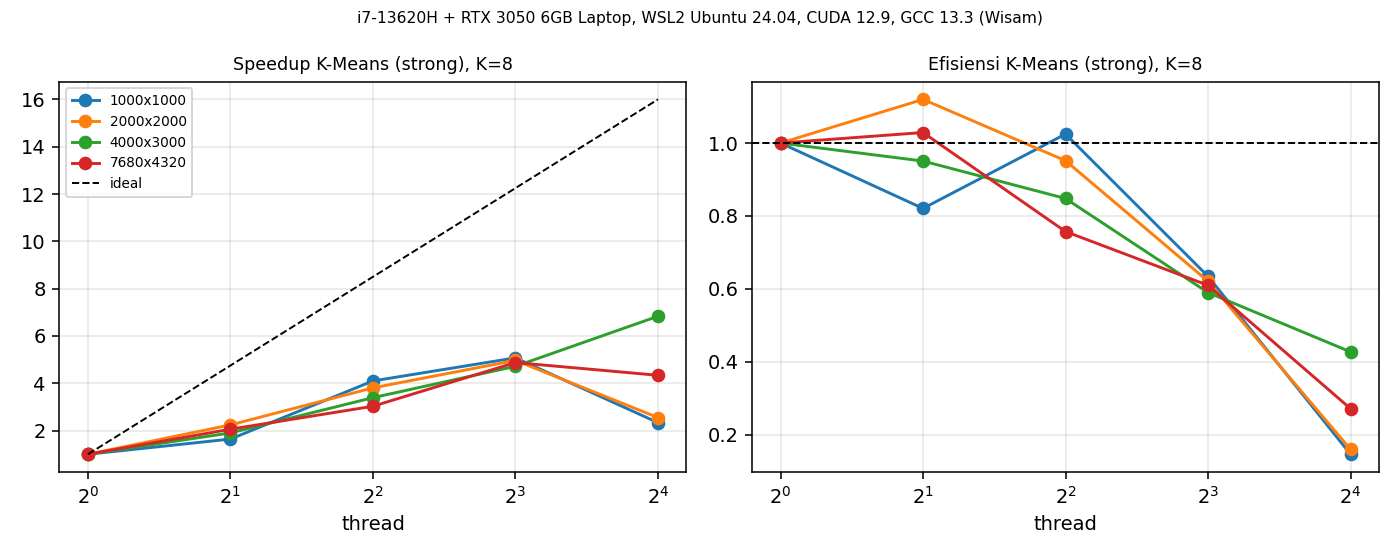
\includegraphics[width=\textwidth]{strong_kmeans_k8.png}
\caption{\emph{Speedup} dan efisiensi K-Means OpenMP (\emph{strong scaling}), $K=8$, citra sintetis, Mesin B. Garis putus-putus = ideal}
\label{fig:strong}
\end{figure}

\textbf{\emph{Weak scaling}.} Pada \emph{weak scaling} (Tabel~\ref{tab:weak}, Gambar~\ref{fig:weak}), beban per \emph{thread} dibuat tetap, sesuai sudut pandang Gustafson \cite{gustafson1988}. Efisiensi K-Means pada $K=8$ masih \WeakKMDua{} dengan 2 \emph{thread}, lalu turun menjadi \WeakKMDelapan{} dengan 8 \emph{thread} dan \WeakKMEnambelas{} dengan 16 \emph{thread}. Efisiensi Total pada 16 \emph{thread} lebih rendah lagi (\WeakTotEnambelas), karena waktu baca PNG serial tumbuh bersama ukuran citra. Jadi menambah \emph{thread} di mesin ini tidak cukup untuk menjaga waktu tetap ketika citra membesar.

% DIBUAT OLEH laporan/skrip/tabel_ke_tex.py -- jangan disunting tangan.
\begin{table}[H]
\centering
\caption{\emph{Weak scaling} OpenMP (beban per \emph{thread} tetap 2 juta piksel), citra sintetis, Mesin B (ms)}
\label{tab:weak}
\footnotesize
\begin{tabularx}{\textwidth}{rL{2.4cm}>{\raggedleft\arraybackslash}X>{\raggedleft\arraybackslash}X>{\raggedleft\arraybackslash}X>{\raggedleft\arraybackslash}X>{\raggedleft\arraybackslash}X>{\raggedleft\arraybackslash}X>{\raggedleft\arraybackslash}X>{\raggedleft\arraybackslash}X}
\hline
\hdr{$T$} & \hdr{Citra} & \hdr{K-M $K{=}4$} & \hdr{$E_w$} & \hdr{Total $K{=}4$} & \hdr{$E_w$} & \hdr{K-M $K{=}8$} & \hdr{$E_w$} & \hdr{Total $K{=}8$} & \hdr{$E_w$} \\ \hline
1 & 2000$\times$1000 & 197,5 & 1,00 & 237,1 & 1,00 & 343,0 & 1,00 & 415,0 & 1,00 \\ \hline
2 & 4000$\times$1000 & 192,4 & 1,03 & 264,0 & 0,90 & 359,0 & 0,96 & 455,1 & 0,91 \\ \hline
4 & 8000$\times$1000 & 257,1 & 0,77 & 389,6 & 0,61 & 461,5 & 0,74 & 626,9 & 0,66 \\ \hline
8 & 16000$\times$1000 & 341,3 & 0,58 & 598,5 & 0,40 & 767,7 & 0,45 & 1100,5 & 0,38 \\ \hline
16 & 32000$\times$1000 & 1038,3 & 0,19 & 1679,0 & 0,14 & 1451,7 & 0,24 & 2148,1 & 0,19 \\ \hline
\end{tabularx}
\par\smallskip\footnotesize\raggedright $E_w = t(T{=}1)/t(T)$, ideal 1. Sumber: \kode{run\_20261127\_1634\_weak\_summary.csv}.
\end{table}


\begin{figure}[H]
\centering
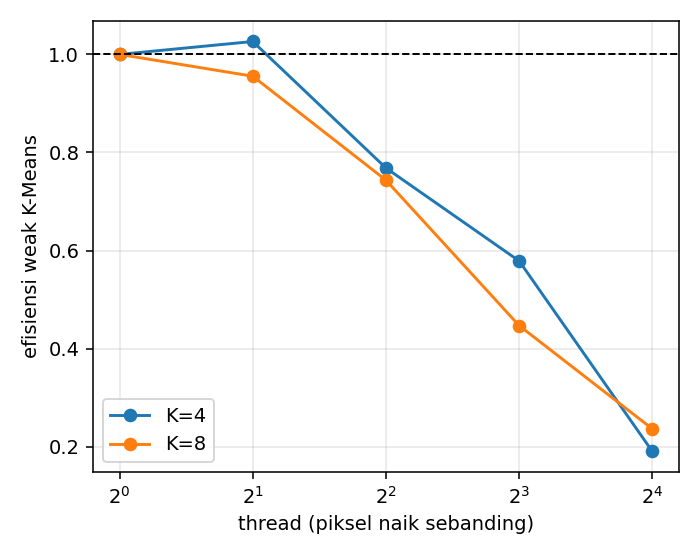
\includegraphics[width=0.55\textwidth]{weak_kmeans.png}
\caption{Efisiensi \emph{weak scaling} K-Means OpenMP, citra sintetis, Mesin B}
\label{fig:weak}
\end{figure}

\section{Kinerja CUDA}
\label{sec:hasilcuda}
\textbf{Rincian waktu.} Tabel~\ref{tab:cudarinci} memecah tahap K-Means CUDA menjadi salin ke GPU (h2d), \emph{kernel}, dan salin kembali (d2h). Pada 7680$\times$4320, $K=8$, rinciannya adalah h2d \HdDelapan~ms, \emph{kernel} \KernelDelapan~ms, dan d2h \DdhDelapan~ms. Pada semua baris, d2h lebih lama daripada h2d (\RasioDdhHdMin--\RasioDdhHdMax). Sebagian selisih ini sesuai dengan ukuran data: label dikirim balik sebagai \kode{int32} (4 \emph{byte} per piksel), sedangkan citra dikirim sebagai 3 \emph{byte} per piksel, atau rasio 4/3. Rasio yang terukur lebih besar daripada itu, dan penyebab sisanya \textbf{tidak diukur} (tanpa Nsight). Transfer hanya terjadi sekali di awal dan sekali di akhir (Subbab~\ref{sec:cuda}), tetapi pada citra besar porsinya tetap besar dibandingkan \emph{kernel} 20 iterasi. Pemanasan konteks CUDA hanya terekam pada 4000$\times$3000; di sana pemanasan lebih lama daripada seluruh tahap K-Means untuk keempat nilai $K$.

% DIBUAT OLEH laporan/skrip/tabel_ke_tex.py -- jangan disunting tangan.
\begin{table}[H]
\centering
\caption{Rincian tahap K-Means CUDA (L1) per citra dan $K$, citra sintetis, Mesin B (ms)}
\label{tab:cudarinci}
\small
\begin{tabularx}{\textwidth}{L{2.3cm}r>{\raggedleft\arraybackslash}X>{\raggedleft\arraybackslash}X>{\raggedleft\arraybackslash}X>{\raggedleft\arraybackslash}X>{\raggedleft\arraybackslash}X}
\hline
\hdr{Citra} & \hdr{$K$} & \hdr{h2d} & \hdr{\emph{Kernel}} & \hdr{d2h} & \hdr{K-Means} & \hdr{Pemanasan} \\ \hline
4000$\times$3000 & 2 & 7,5 & 25,6 & 24,0 & 57,4 & 191 \\ \hline
4000$\times$3000 & 4 & 11,3 & 26,0 & 22,5 & 59,6 & 195 \\ \hline
1000$\times$1000 & 8 & 0,8 & 2,1 & 2,0 & 4,8 & -- \\ \hline
2000$\times$2000 & 8 & 2,9 & 7,7 & 8,0 & 18,5 & -- \\ \hline
4000$\times$3000 & 8 & 7,8 & 23,4 & 24,1 & 55,7 & 194 \\ \hline
7680$\times$4320 & 8 & 21,6 & 53,7 & 62,1 & 138,9 & -- \\ \hline
4000$\times$3000 & 16 & 9,2 & 21,9 & 23,6 & 59,7 & 214 \\ \hline
\end{tabularx}
\par\smallskip\footnotesize\raggedright h2d/\emph{kernel}/d2h diukur dengan CUDA \emph{events}. Pemanasan = inisialisasi konteks CUDA (\kode{warmup\_ms}), di luar \kode{total\_ms}; ``--'' = tidak direkam pada sesi \kode{bench\_gpu}.
\end{table}


\textbf{Pengaruh $K$.} Pada 4000$\times$3000 (Tabel~\ref{tab:pengaruhk}), K-Means L0 tumbuh \RasioKLo{} dari $K=2$ ke $K=16$, mendekati linear terhadap $K$. K-Means CUDA hampir datar (\RasioKCuda). Tabel~\ref{tab:cudarinci} menunjukkan bahwa waktu \emph{kernel} sendiri juga hampir tidak berubah terhadap $K$ (\KernelKMin--\KernelKMax~ms untuk $K=2$ sampai 16). Dugaan yang \textbf{tidak diukur}: \emph{kernel} dibatasi akses memori (membaca citra dan menulis label), bukan perhitungan jarak yang sebanding dengan $K$. Akibatnya, \emph{speedup} K-Means CUDA membesar bersama $K$ dan mencapai \LdSKMEnambelas{} pada $K=16$.

% DIBUAT OLEH laporan/skrip/tabel_ke_tex.py -- jangan disunting tangan.
\begin{table}[H]
\centering
\caption{Waktu K-Means (ms) terhadap $K$ pada 4000$\times$3000, citra sintetis, Mesin B (dalam kurung: rasio terhadap $K=2$)}
\label{tab:pengaruhk}
\small
\begin{tabularx}{\textwidth}{L{2.6cm}>{\raggedleft\arraybackslash}X>{\raggedleft\arraybackslash}X>{\raggedleft\arraybackslash}X>{\raggedleft\arraybackslash}X}
\hline
\hdr{Konfigurasi} & \hdr{$K=2$} & \hdr{$K=4$} & \hdr{$K=8$} & \hdr{$K=16$} \\ \hline
L0 & 640,7 (1,00\ensuremath{\times}) & 1017,2 (1,59\ensuremath{\times}) & 2385,1 (3,72\ensuremath{\times}) & 4794,6 (7,48\ensuremath{\times}) \\ \hline
L2 (8 thr) & 197,0 (1,00\ensuremath{\times}) & 292,2 (1,48\ensuremath{\times}) & 488,5 (2,48\ensuremath{\times}) & 907,0 (4,61\ensuremath{\times}) \\ \hline
L2 (16 thr) & 256,7 (1,00\ensuremath{\times}) & 376,1 (1,46\ensuremath{\times}) & 337,3 (1,31\ensuremath{\times}) & 684,2 (2,67\ensuremath{\times}) \\ \hline
L1 & 57,4 (1,00\ensuremath{\times}) & 59,6 (1,04\ensuremath{\times}) & 55,7 (0,97\ensuremath{\times}) & 59,7 (1,04\ensuremath{\times}) \\ \hline
L1+L2 (8 thr) & 63,5 (1,00\ensuremath{\times}) & 69,6 (1,09\ensuremath{\times}) & 55,4 (0,87\ensuremath{\times}) & 53,7 (0,84\ensuremath{\times}) \\ \hline
\end{tabularx}
\par\smallskip\footnotesize\raggedright Sumber: \kode{run\_20261127\_1634\_ksweep\_summary.csv}.
\end{table}


\textbf{\emph{Throughput}.} Tabel~\ref{tab:throughput} menunjukkan bahwa CUDA memproses \TpCudaMin--\TpCudaMax~ns per piksel per iterasi pada $K=8$ di semua ukuran. Angka yang datar ini berarti waktu K-Means CUDA tumbuh linear terhadap jumlah piksel pada rentang yang diukur.

% DIBUAT OLEH laporan/skrip/tabel_ke_tex.py -- jangan disunting tangan.
\begin{table}[H]
\centering
\caption{\emph{Throughput} K-Means dalam ns per piksel per iterasi, $K=8$, citra sintetis, Mesin B}
\label{tab:throughput}
\small
\begin{tabularx}{\textwidth}{L{2.6cm}>{\raggedleft\arraybackslash}X>{\raggedleft\arraybackslash}X>{\raggedleft\arraybackslash}X>{\raggedleft\arraybackslash}X}
\hline
\hdr{Citra} & \hdr{Piksel (juta)} & \hdr{L0} & \hdr{L2 (8 thr)} & \hdr{L1} \\ \hline
1000$\times$1000 & 1,00 & 10,37 & 2,17 & 0,24 \\ \hline
2000$\times$2000 & 4,00 & 9,72 & 2,06 & 0,23 \\ \hline
4000$\times$3000 & 12,00 & 9,94 & 2,04 & 0,23 \\ \hline
7680$\times$4320 & 33,18 & 8,85 & 1,90 & 0,21 \\ \hline
\end{tabularx}
\par\smallskip\footnotesize\raggedright ns/piksel/iterasi = \kode{kmeans\_ms}$\times10^6$/(piksel$\times$iterasi). Sumber: \kode{docs/BENCH\_scaling\_mesin\_wisam.md} bagian 5 (dihitung ulang dari CSV).
\end{table}


\textbf{Varian \emph{kernel}.} Tabel~\ref{tab:variancuda} membandingkan tiga varian pada tahap K-Means saja, diukur dengan \kode{tests/bench\_cuda} di luar \kode{landcover}. Reduksi di \emph{shared memory} (T4) \TempatTigaMin--\TempatTigaMax{} lebih cepat daripada \kode{atomicAdd} global (T3). Hasil ini sesuai dengan alasan rancangan T4 (Subbab~\ref{sec:cuda}): pada T3 semua \emph{thread} menulis ke akumulator global yang sama, sedangkan T4 menjumlahkan dulu per \emph{block}. Penyebab ini tidak diprofilkan. Varian \emph{streams} dengan \emph{pinned memory} (T5) \LimaEmpatMin--\LimaEmpatMax{} lebih lambat daripada T4 pada semua ukuran yang diukur. Dugaan yang \textbf{tidak diukur}: tumpang tindih transfer pada T5 hanya terjadi di iterasi pertama dan terakhir (Subbab~\ref{sec:bersamaan}), sehingga keuntungannya tidak menutup biaya pembagian potongan dan sinkronisasi \emph{stream}. Pengaruh T5 pada \emph{pipeline} utuh \textbf{tidak diukur}, karena \kode{landcover} hanya memanggil T4.

% DIBUAT OLEH laporan/skrip/tabel_ke_tex.py -- jangan disunting tangan.
\begin{table}[H]
\centering
\caption{Varian CUDA pada tahap K-Means saja (\kode{tests/bench\_cuda}, citra acak), Mesin B (ms)}
\label{tab:variancuda}
\small
\begin{tabularx}{\textwidth}{L{2.3cm}r>{\raggedleft\arraybackslash}X>{\raggedleft\arraybackslash}X>{\raggedleft\arraybackslash}X>{\raggedleft\arraybackslash}X>{\raggedleft\arraybackslash}X}
\hline
\hdr{Ukuran} & \hdr{$K$} & \hdr{T3 \emph{simple}} & \hdr{T4 \emph{shared}} & \hdr{T5 \emph{streams}} & \hdr{T4 vs T3} & \hdr{T5 vs T3} \\ \hline
1000$\times$1000 & 4 & 48,0 & 2,8 & 4,2 & 16,9\ensuremath{\times} & 11,4\ensuremath{\times} \\ \hline
1000$\times$1000 & 8 & 39,6 & 3,0 & 3,7 & 13,2\ensuremath{\times} & 10,6\ensuremath{\times} \\ \hline
1000$\times$1000 & 16 & 29,1 & 3,1 & 4,3 & 9,5\ensuremath{\times} & 6,7\ensuremath{\times} \\ \hline
2000$\times$2000 & 8 & 154,1 & 9,7 & 11,6 & 15,9\ensuremath{\times} & 13,3\ensuremath{\times} \\ \hline
4000$\times$3000 & 4 & 450,8 & 30,3 & 39,8 & 14,9\ensuremath{\times} & 11,3\ensuremath{\times} \\ \hline
4000$\times$3000 & 8 & 462,6 & 30,6 & 43,6 & 15,1\ensuremath{\times} & 10,6\ensuremath{\times} \\ \hline
4000$\times$3000 & 16 & 317,4 & 31,5 & 40,7 & 10,1\ensuremath{\times} & 7,8\ensuremath{\times} \\ \hline
7680$\times$4320 & 4 & 1233,5 & 91,3 & 96,4 & 13,5\ensuremath{\times} & 12,8\ensuremath{\times} \\ \hline
7680$\times$4320 & 8 & 1277,8 & 98,1 & 101,0 & 13,0\ensuremath{\times} & 12,7\ensuremath{\times} \\ \hline
7680$\times$4320 & 16 & 888,0 & 89,6 & 95,6 & 9,9\ensuremath{\times} & 9,3\ensuremath{\times} \\ \hline
\end{tabularx}
\par\smallskip\footnotesize\raggedright Diukur di luar \kode{landcover} (tanpa baca/tulis PNG). Sumber: \kode{run\_20261127\_1634\_cudavar\_summary.csv}.
\end{table}


\section{Ambang Mode Otomatis}
\label{sec:hasilambang}
Tabel~\ref{tab:ambang} membandingkan OpenMP dan CUDA pada \AmbJumlah{} konfigurasi (citra sintetis $N$ sampai \AmbNMax{} juta piksel, $K$ = 4, 8, 16). Menurut Total, CUDA unggul pada \AmbCudaTotal{} dari \AmbJumlah{} konfigurasi. Menurut Proses, CUDA hanya unggul pada \AmbCudaProses{} konfigurasi, karena pemanasan konteks CUDA (\AmbWarmMin--\AmbWarmMax~ms pada sesi ini) lebih besar daripada keuntungan K-Means pada citra kecil dan $K$ kecil.

% DIBUAT OLEH laporan/skrip/tabel_ke_tex.py -- jangan disunting tangan.
\begin{table}[H]
\centering
\caption{Pemenang OpenMP vs CUDA menurut Total dan menurut Proses pada 21 konfigurasi, citra sintetis, Mesin B (ms)}
\label{tab:ambang}
\footnotesize
\begin{tabularx}{\textwidth}{rr>{\raggedleft\arraybackslash}X>{\raggedleft\arraybackslash}X>{\raggedleft\arraybackslash}X>{\raggedleft\arraybackslash}X>{\raggedleft\arraybackslash}X>{\raggedleft\arraybackslash}X>{\raggedleft\arraybackslash}X>{\raggedleft\arraybackslash}X}
\hline
\hdr{$N$ (juta)} & \hdr{$K$} & \hdr{$N{\times}K$ (juta)} & \hdr{omp Total} & \hdr{cuda Total} & \hdr{Unggul} & \hdr{omp Proses} & \hdr{cuda Proses} & \hdr{Unggul} & \hdr{Aturan} \\ \hline
0,10 & 4 & 0,4 & 7,0 & 4,6 & cuda & 40,6 & 291,3 & omp & omp \\ \hline
0,41 & 4 & 1,6 & 20,2 & 11,2 & cuda & 43,9 & 268,3 & omp & omp \\ \hline
1,00 & 4 & 4,0 & 40,9 & 26,1 & cuda & 68,1 & 265,1 & omp & omp \\ \hline
4,00 & 4 & 16,0 & 168,0 & 87,4 & cuda & 207,0 & 351,9 & omp & omp \\ \hline
6,25 & 4 & 25,0 & 231,0 & 138,3 & cuda & 267,1 & 554,8 & omp & omp \\ \hline
9,00 & 4 & 36,0 & 333,8 & 187,0 & cuda & 370,1 & 447,9 & omp & omp \\ \hline
12,00 & 4 & 48,0 & 432,5 & 248,1 & cuda & 469,9 & 554,0 & omp & omp \\ \hline
0,10 & 8 & 0,8 & 10,2 & 5,9 & cuda & 39,4 & 251,2 & omp & omp \\ \hline
0,41 & 8 & 3,3 & 34,9 & 19,3 & cuda & 71,1 & 278,8 & omp & omp \\ \hline
1,00 & 8 & 8,0 & 70,7 & 37,6 & cuda & 112,1 & 303,6 & omp & omp \\ \hline
4,00 & 8 & 32,0 & 242,6 & 105,8 & cuda & 298,7 & 398,7 & omp & omp \\ \hline
6,25 & 8 & 50,0 & 371,6 & 153,9 & cuda & 421,3 & 444,6 & omp & omp \\ \hline
9,00 & 8 & 72,0 & 538,3 & 218,1 & cuda & 601,7 & 517,6 & cuda & cuda \\ \hline
12,00 & 8 & 96,0 & 703,5 & 276,1 & cuda & 765,0 & 599,7 & cuda & cuda \\ \hline
0,10 & 16 & 1,6 & 14,3 & 5,8 & cuda & 36,0 & 230,6 & omp & omp \\ \hline
0,41 & 16 & 6,6 & 56,6 & 23,0 & cuda & 100,4 & 296,1 & omp & omp \\ \hline
1,00 & 16 & 16,0 & 131,0 & 50,8 & cuda & 203,3 & 319,3 & omp & omp \\ \hline
4,00 & 16 & 64,0 & 421,3 & 124,2 & cuda & 496,0 & 573,8 & omp & omp \\ \hline
6,25 & 16 & 100,0 & 627,4 & 171,2 & cuda & 696,7 & 506,3 & cuda & cuda \\ \hline
9,00 & 16 & 144,0 & 896,6 & 247,7 & cuda & 983,5 & 563,0 & cuda & cuda \\ \hline
12,00 & 16 & 192,0 & 1151,2 & 305,5 & cuda & 1224,7 & 658,3 & cuda & cuda \\ \hline
\end{tabularx}
\par\smallskip\footnotesize\raggedright omp = \kode{L2 omp x8}; cuda = yang tercepat dari L1 dan L1+L2 (8 \emph{thread}) untuk kriteria itu. Proses = waktu dinding, termasuk pemanasan CUDA. Aturan = pilihan $N\times K\geq70$ juta. Sumber: \kode{bench/results/ambang\_summary.csv} (\kode{bench/fit\_auto\_threshold.py}).
\end{table}


Aturan yang diuji:
\begin{itemize}
    \item \textbf{Aturan lama} ($N\geq100.000$ piksel, diturunkan dari Total) memilih yang tercepat menurut Proses hanya pada \AmbLamaBenarProses{} dari \AmbJumlah{} konfigurasi, dengan kerugian \AmbLamaRugi~ms.
    \item \textbf{Selalu OpenMP} benar pada \AmbOmpBenarProses{} konfigurasi, dengan kerugian \AmbOmpRugi~ms.
    \item \textbf{Aturan baru} $N\times K\geq70$ juta (Persamaan~\ref{eq:ambang}) benar pada \AmbBaruBenarProses{} dari \AmbJumlah{} konfigurasi, dengan kerugian \AmbBaruRugi~ms.
\end{itemize}
Aturan baru memakai $N\times K$, bukan $N$ saja, karena waktu K-Means OpenMP sebanding dengan $N\times K$, sedangkan K-Means CUDA hampir tidak bergantung pada $K$ (Tabel~\ref{tab:pengaruhk}). Aturan ini hanya berlaku untuk mesin, data, dan cara pemanggilan yang diukur. Bila aplikasi kelak memakai proses CUDA yang menetap, sehingga pemanasan dibayar sekali, ambang harus dihitung ulang dengan Total.

\section{Verifikasi Hasil Identik}
\label{sec:hasilverifikasi}
Tabel~\ref{tab:verifikasi} merangkum semua pemeriksaan kesamaan hasil antarmode. Pemeriksaan pada kolom ``Identik'' \emph{benchmark} hanya membandingkan \emph{centroid} dan \emph{counts}. Kesamaan label per piksel dibuktikan oleh program uji inti dan oleh \kode{cmp} pada \kode{labels.u8}.

\begin{table}[H]
\centering
\caption{Ringkasan verifikasi hasil identik antarmode}
\label{tab:verifikasi}
\small
\begin{tabularx}{\textwidth}{L{3.3cm}YL{3.4cm}L{2.5cm}}
\hline
\hdr{Uji} & \hdr{Yang dibandingkan} & \hdr{Cakupan} & \hdr{Hasil} \\ \hline
\kode{test\_ref} & Implementasi acuan C++ & Kasus uji inti & 0 kegagalan \\ \hline
\kode{test\_cuda\_vs\_ref} & Label dan \emph{centroid} CUDA vs serial & 615 kasus (ukuran, $K$, \emph{seed}) & 615 dari 615 lulus \\ \hline
\kode{test\_omp\_vs\_cpu} & Label dan \emph{centroid} OpenMP vs serial & Kasus uji OpenMP & Semua sama \\ \hline
\kode{test\_png\_omp} & PNG paralel vs serial & Berkas PNG keluaran & Lulus (\emph{exit} 0) \\ \hline
Kolom ``Identik'' \emph{benchmark} & \emph{Centroid} dan \emph{counts} vs L0 & \IdentikJumlah{} baris ringkasan \emph{benchmark} Mesin B (sintetis) & \IdentikYa{} dari \IdentikJumlah{} identik \\ \hline
\kode{cmp} Sentinel-2 (25 Nov) & \kode{labels.u8}, \emph{centroid}, \emph{counts}: cpu vs cuda & 512, 1024, 2048 px $\times$ $K$ = 4, 8, 16 & 9 dari 9 identik \\ \hline
\kode{cmp} Sentinel-2 (28 Nov) & \kode{labels.u8}, \emph{centroid}, \emph{counts}: cpu vs omp dan cpu vs cuda & 2048 px, $K=8$, biner \kode{main} & \CmpSama{} dari \CmpSama{} berkas identik \\ \hline
Aplikasi (halaman Kinerja) & \kode{labels.u8} penuh, \emph{centroid}, \emph{counts} & Sentinel-2 2048 px, $K=8$ & ``Label identik 100\%'' \\ \hline
\kode{pytest} (Windows) & Logika aplikasi & Seluruh \emph{suite} & 1000 lulus, 41 dilewati, 1 gagal* \\ \hline
Tes biner nyata & Aplikasi + \kode{landcover} asli & Lewat pembungkus WSL & 36 lulus, 3 dilewati \\ \hline
\end{tabularx}
\par\smallskip\footnotesize\raggedright *Tes batas waktu 1 detik yang peka beban mesin; diulang tersendiri, lulus 3 dari 3. Tes yang dilewati hanya berlaku bila OpenMP/CUDA \emph{tidak} terhubung. Sumber: uji 28 Nov pada \kode{main} \kode{f78b5d4} (Mesin C), \kode{bench/results/*\_summary.csv}, dan \kode{laporan/hasil\_s2/cmp.txt}.
\end{table}

Hasilnya identik pada semua pemeriksaan. Ini sesuai rancangan pada Subbab~\ref{sec:konsistensi}: aritmetika integer, pembagian dibulatkan ke bawah, aturan seri yang sama, dan \emph{centroid} awal yang dihitung sekali di CPU. Karena labelnya identik, persentase dan luas setiap kelas pada kedua mode juga identik, dan selisih waktu di subbab sebelumnya murni berasal dari optimasi.

\section{Hasil Aplikasi pada Sentinel-2}
\label{sec:hasilsentinel}
Gambar~\ref{fig:s2peta} menampilkan potongan Sentinel-2 T49MDM 2048$\times$2048 piksel (\SPiksel{} piksel) dan peta kelompok hasil K-Means dengan $K=8$, 20 iterasi, dan \emph{seed} 42. Peta ini dibuat oleh \kode{landcover} versi \kode{main}; mode cpu, omp, dan cuda menghasilkan \kode{labels.u8} yang identik (Tabel~\ref{tab:verifikasi}). Sebanyak \SNodataPiksel{} piksel (\SNodataPersen) adalah \emph{nodata} $(0,0,0)$ pada baji di tepi kanan potongan. Seluruh piksel itu jatuh ke kelompok \SKelompokNodata{} dan dikecualikan dari persen dan luas.

\begin{figure}[H]
\centering
\begin{minipage}{0.48\textwidth}\centering
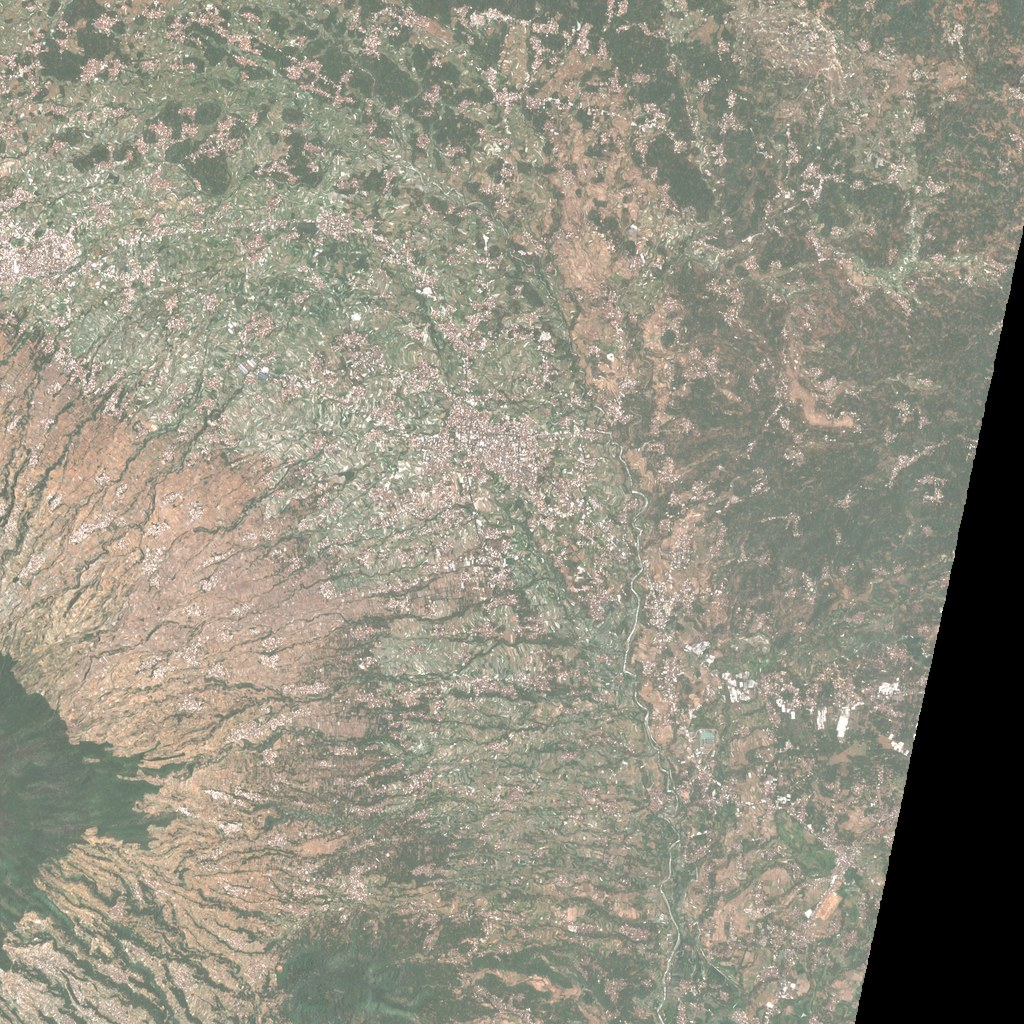
\includegraphics[width=\textwidth]{s2_mdm2048_asli.jpg}\\[2pt]
\small (a) Citra asli (B04/B03/B02)
\end{minipage}\hfill
\begin{minipage}{0.48\textwidth}\centering
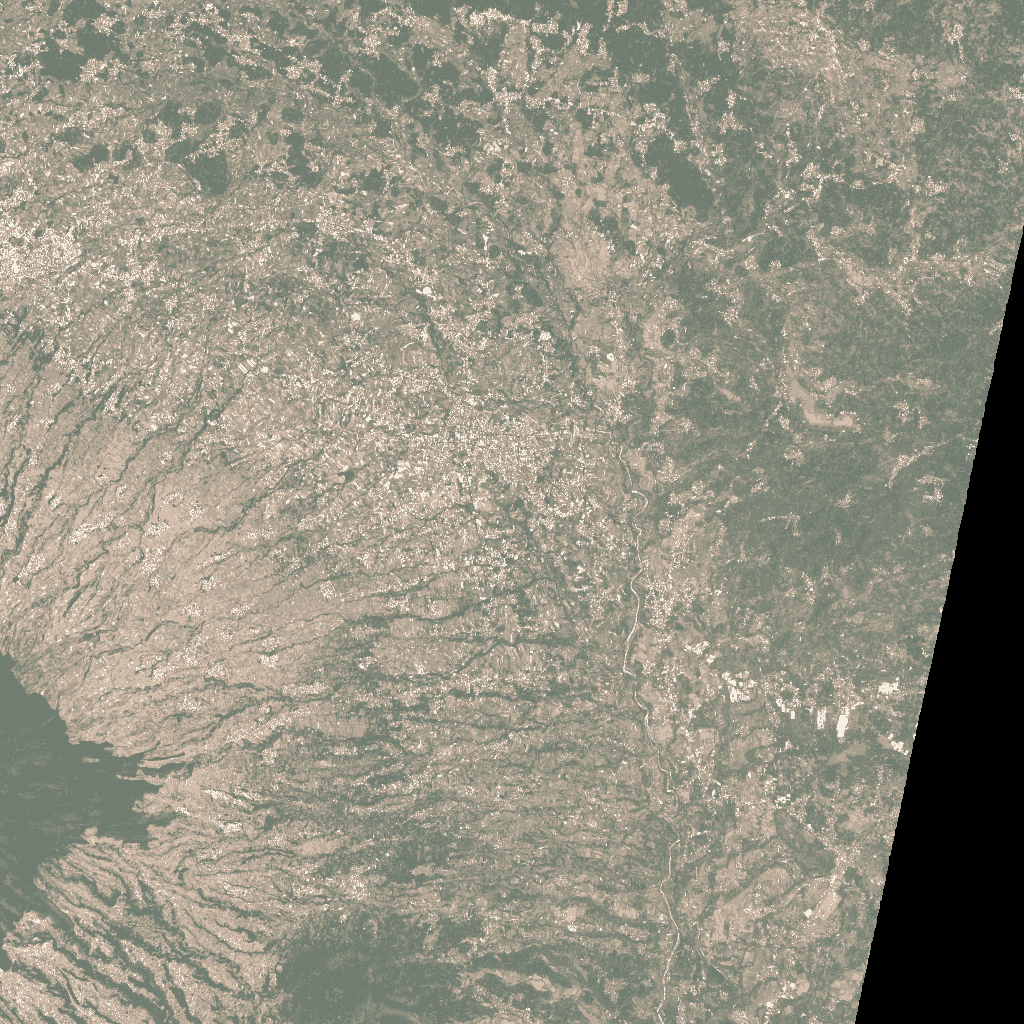
\includegraphics[width=\textwidth]{s2_mdm2048_peta_k8.png}\\[2pt]
\small (b) Peta kelompok, $K=8$
\end{minipage}
\caption{Sentinel-2 T49MDM 2048$\times$2048 px dan peta hasil K-Means. Setiap piksel diwarnai dengan warna \emph{centroid} kelompoknya; gambar diperkecil menjadi 1024 px untuk laporan}
\label{fig:s2peta}
\end{figure}

Tabel~\ref{tab:luass2} menunjukkan persentase dan luas setelah delapan kelompok diberi nama dan digabung menjadi empat kelas di halaman Pemetaan. Total luas valid adalah \SValidHa~ha. Penamaan ini dilakukan manual dari warna \emph{centroid} dan kenampakan visual, sehingga tabel ini adalah contoh keluaran aplikasi, bukan hasil klasifikasi yang tervalidasi.

% DIBUAT OLEH laporan/skrip/tabel_ke_tex.py -- jangan disunting tangan.
\begin{table}[H]
\centering
\caption{Persentase dan luas per kelas, Sentinel-2 T49MDM 2048$\times$2048 px, $K=8$}
\label{tab:luass2}
\small
\begin{tabularx}{\textwidth}{L{2.9cm}Y>{\raggedleft\arraybackslash}p{2.1cm}>{\raggedleft\arraybackslash}p{1.6cm}>{\raggedleft\arraybackslash}p{1.9cm}}
\hline
\hdr{Kelas} & \hdr{Kelompok (\emph{centroid} R,G,B)} & \hdr{Piksel} & \hdr{Persen} & \hdr{Luas (ha)} \\ \hline
Vegetasi & 2 (114,125,113), 5 (126,134,120), 6 (144,145,129) & 1.945.270 & 49,58\% & 19.452,70 \\ \hline
Lahan terbuka & 0 (186,170,153), 3 (211,191,172) & 1.074.523 & 27,38\% & 10.745,23 \\ \hline
Lahan terbangun & 1 (246,239,228) & 114.105 & 2,91\% & 1.141,05 \\ \hline
Lainnya & 4 (164,157,140) & 789.986 & 20,13\% & 7.899,86 \\ \hline
\textbf{Total valid} &  & 3.923.884 & 100,00\% & 39.238,84 \\ \hline
\emph{Nodata} (dikecualikan) & 7 (0,0,0) & 270.420 & 6,45\% & 2.704,20 \\ \hline
\end{tabularx}
\par\smallskip\footnotesize\raggedright Persen kelas dihitung dari piksel valid; persen \emph{nodata} dari seluruh citra. 1 piksel = 10 m $\times$ 10 m. Nama kelas diberikan manual dari warna \emph{centroid} dan kenampakan visual (bukan klasifikasi terverifikasi). Sumber: \kode{laporan/hasil\_s2/} (\kode{counts.json}, \kode{meta\_cpu.json}, \kode{kelas.json}); Mesin C.
\end{table}


Beberapa kasus sulit terlihat karena hanya tiga kanal tampak yang dipakai (tanpa NIR/SWIR):
\begin{enumerate}
    \item \textbf{Air dan bayangan.} Pada $K=8$ tidak terbentuk kelompok air tersendiri. Koridor sungai dan bayangan lereng masuk ke kelompok vegetasi gelap (kelompok 2 dan 5), sehingga kelas Air tidak dibuat.
    \item \textbf{Permukiman dan tanah terbuka.} Atap terang (kelompok 1) berdekatan secara spektral dengan tanah kering dan kabut tipis (kelompok 3). Kelompok 4 mencampur lahan terasering, jalan, dan tepi vegetasi, sehingga diberi nama ``Lainnya''.
    \item \textbf{Kelompok kosong.} Pada $K=16$ dengan \emph{seed} yang sama, beberapa \emph{centroid} awal jatuh pada piksel \emph{nodata} $(0,0,0)$. Tiga \emph{centroid} awal bernilai $(0,0,0)$; dua di antaranya (kelompok 9 dan 12) berakhir dengan nol piksel, sehingga kelompok bukan-\emph{nodata} yang berisi tinggal 13, bukan 15. Perilaku ini sah menurut kontrak (kelompok kosong dipertahankan dan ditampilkan 0\%), tetapi menunjukkan bahwa \emph{nodata} sebaiknya dikeluarkan sebelum inisialisasi bila hasil $K$ besar dibutuhkan.
\end{enumerate}

Waktu \emph{run} Sentinel-2 di Mesin C tidak dilaporkan sebagai hasil kinerja, karena hanya berupa uji fungsional (satu \emph{run} per konfigurasi, mesin berbeda, citra lebih kecil daripada citra pengukuran utama).

\section{Hipotesis dan Analisis Amdahl}
\label{sec:hipotesis}
Tabel~\ref{tab:hipotesis} membandingkan hipotesis Subbab~\ref{sec:hipotesisawal} dengan data terdekat dari Mesin B.

\begin{table}[H]
\centering
\caption{Hipotesis dan hasil pengukuran (Mesin B, citra sintetis, kecuali H4)}
\label{tab:hipotesis}
\small
\begin{tabularx}{\textwidth}{L{3.2cm}YL{3.5cm}}
\hline
\hdr{Hipotesis} & \hdr{Data terdekat} & \hdr{Kesimpulan} \\ \hline
H1: K-Means mengambil porsi terbesar pada L0 & Porsi K-Means \PorsiKMLoMin--\PorsiKMLoMax{} di Mesin B (Tabel~\ref{tab:l0b}) dan \PorsiKMAMin--\PorsiKMAMax{} di Mesin A (Tabel~\ref{tab:l0a}) & Terbukti pada kedua mesin \\ \hline
H2a: K-Means CUDA $\geq20\times$ (4096$^2$, $K=8$) & 4096$^2$ tidak diukur. Ukuran terdekat 4000$\times$3000 (12 juta piksel, bukan 16,8 juta): \LdSKMEmpat. Semua ukuran $K=8$: \HDuaCudaMin--\HDuaCudaMax{} (Tabel~\ref{tab:bertahapk8}) & Tercapai pada ukuran terdekat \\ \hline
H2b: K-Means OpenMP 8 \emph{thread} $\geq4\times$ & Terhadap L0, $K=8$: \HDuaOmpMin--\HDuaOmpMax{} di semua ukuran; terhadap OpenMP 1 \emph{thread} pada 4000$\times$3000: \HDuaOmpSatuEmpat. Pada 4000$\times$3000: $K=2$ \HDuaOmpKDua, $K=4$ \HDuaOmpKEmpat, $K=16$ \HDuaOmpKEnambelas & Tercapai pada $K=8$ (kondisi hipotesis); tidak tercapai pada $K\leq4$ \\ \hline
H3: \emph{End-to-end} satu \emph{tile} penuh $\geq5\times$ & \emph{Tile} penuh tidak diukur. 7680$\times$4320, $K=8$: Total \LdLdSTotalDelapan, Proses tidak diukur. 4000$\times$3000, $K=8$: Total \LdLdSTotalEmpat, Proses \SProsesTerbaikKDelapan{} (konfigurasi tercepat); $K=16$: Proses \SProsesTerbaikKEnambelas & Tidak dapat disimpulkan untuk \emph{tile} penuh. Pada 12 juta piksel, $K=8$: tercapai menurut Total, tidak menurut Proses \\ \hline
H4: Label identik 100\% & \kode{test\_cuda\_vs\_ref}, \kode{test\_omp\_vs\_cpu}, \kode{cmp} \kode{labels.u8} Sentinel-2 cpu vs omp vs cuda (Tabel~\ref{tab:verifikasi}) & Terbukti \\ \hline
\end{tabularx}
\end{table}

\textbf{Analisis Amdahl.} Pada L0 7680$\times$4320, $K=8$, porsi K-Means adalah $q=\AmdP$. Bila hanya K-Means yang dipercepat tanpa batas, Persamaan~\ref{eq:amdahl} dengan fraksi serial $f=1-q$ dan $p\to\infty$ memberi batas \emph{speedup} total $1/(1-q)\approx\AmdBatas$ \cite{amdahl1967}. Hasil pengukuran sesuai dengan analisis ini:
\begin{enumerate}
    \item L1 saja mempercepat K-Means \LdSKMDelapan, tetapi Total hanya membaik \LdSTotalDelapan, mendekati batas \AmdBatas. Tahap lain belum disentuh, sehingga mempercepat K-Means lebih jauh hampir tidak berguna.
    \item L1+L2 mencapai \LdLdSTotalDelapan, melampaui batas tersebut, karena L2 juga memangkas tahap di luar K-Means (pewarnaan dan tulis PNG). Dengan demikian fraksi serialnya mengecil dan batasnya bergeser. Ini menunjukkan mengapa setiap tahap perlu ditempatkan di perangkat terbaiknya, bukan hanya K-Means.
    \item Sesudah L1+L2, K-Means tinggal \PorsiKMLdLdDelapan{} dari Total, sedangkan baca PNG serial menjadi tahap terbesar (\PorsiBacaLdLdDelapan). Bahkan bila K-Means menjadi nol, Total hanya bisa membaik \AmdBatasLdLd{} lagi. Baca PNG adalah \emph{bottleneck} berikutnya.
\end{enumerate}

\section{Batasan}
\label{sec:batasan}
\begin{enumerate}
    \item \textbf{\emph{Tile} penuh tidak diuji.} Data Sentinel-2 yang tersedia hanya potongan sampai 2048 piksel; \emph{tile} 10980$\times$10980 (sekitar 120 juta piksel) tidak ada. Hasil terbesar yang diukur adalah citra sintetis 7680$\times$4320 (sekitar 33 juta piksel), dan H3 tidak dapat disimpulkan untuk \emph{tile} penuh.
    \item \textbf{Kinerja hanya pada citra sintetis.} Waktu baca dan tulis PNG bergantung pada isi citra (kompresi), sehingga angka baca/tulis citra sintetis tidak otomatis berlaku untuk citra satelit.
    \item \textbf{L3 hanya di tingkat \emph{kernel}.} Varian \emph{streams} diukur dengan \kode{tests/bench\_cuda} dan tidak dipanggil \kode{landcover}. Pemrosesan banyak wilayah sekaligus belum dibuat.
    \item \textbf{Proses tidak lengkap.} Waktu dinding proses hanya terekam pada sesi 4000$\times$3000 dan sesi ambang; untuk 1000$^2$, 2000$^2$, dan 7680$\times$4320 hanya Total yang tersedia.
    \item \textbf{Satu mesin acuan dan lima ulangan.} Semua angka kinerja berasal dari satu laptop (Mesin B) dengan skema daya \emph{Balanced} dan median lima ulangan. Dua sesi ukur di mesin yang sama tidak menghasilkan angka yang identik, sehingga selisih kecil antarkonfigurasi (misalnya 8 dan 16 \emph{thread}) belum tentu bermakna.
    \item \textbf{Tanpa Nsight.} Penyebab turunnya efisiensi OpenMP di atas 8 \emph{thread} dan rincian \emph{kernel} CUDA tidak diprofilkan.
    \item \textbf{Segmentasi tanpa pengawasan.} Hasil aplikasi adalah segmentasi awal dari tiga kanal tampak, bukan klasifikasi tutupan lahan yang akurat. Penamaan kelas manual dan tidak divalidasi dengan data lapangan.
\end{enumerate}

% bab6.tex - Kesimpulan dan Saran.
% Semua angka kinerja memakai makro dari tabel/angka.tex (dibuat skrip/tabel_ke_tex.py).
\chapter{KESIMPULAN DAN SARAN}

\section{Kesimpulan}
Berdasarkan hasil pada Bab~V, tiga rumusan masalah pada Bab~I dijawab sebagai berikut.
\begin{enumerate}
    \item \textbf{Peta awal dari citra beresolusi tinggi.} Proyek ini menghasilkan aplikasi pemetaan tutupan lahan yang utuh. Antarmuka web memanggil program inti \kode{landcover}, lalu menampilkan peta kelompok, pelabelan kelas, serta persentase dan luas setiap kelas. Pada potongan Sentinel-2 T49MDM 2048$\times$2048 piksel, aplikasi menghasilkan peta dengan $K=8$ dan tabel luas untuk \SValidHa~ha lahan valid (Subbab~\ref{sec:hasilsentinel}). Pada citra sintetis terbesar yang diukur (7680$\times$4320, sekitar 33 juta piksel, $K=8$), mode Optimalisasi menurunkan Total dari \LoTotalDelapan~ms menjadi \LdLdTotalDelapan~ms. Total ini tidak memuat pemanasan konteks CUDA (\WarmMin--\WarmMax~ms pada sesi pengukuran), dan waktu Proses untuk ukuran ini tidak terekam. Satu \emph{tile} penuh (sekitar 120 juta piksel) tidak diuji karena datanya tidak tersedia. Karena itu, apakah satu \emph{tile} cukup cepat untuk dicoba secara interaktif dengan beberapa nilai $K$ belum dapat disimpulkan.
    \item \textbf{\emph{Bottleneck} dan penempatan tahap.} \emph{Profiling} L0 menunjukkan bahwa K-Means adalah \emph{bottleneck} utama, dengan porsi \PorsiKMLoMin--\PorsiKMLoMax{} dari Total di Mesin B dan \PorsiKMAMin--\PorsiKMAMax{} di Mesin A (Subbab~\ref{sec:profil}). Penempatan akhir setiap tahap ditunjukkan pada Tabel~\ref{tab:penempatan}: K-Means berjalan di CUDA bila $N\times K\geq70$ juta dan di OpenMP bila kurang dari itu; \emph{counts}, pewarnaan, dan tulis PNG memakai OpenMP; baca PNG dan inisialisasi tetap serial. Aturan $N\times K$ memilih konfigurasi tercepat menurut Proses pada \AmbBaruBenarProses{} dari \AmbJumlah{} konfigurasi uji, sedangkan aturan lama hanya pada \AmbLamaBenarProses{} konfigurasi (Subbab~\ref{sec:hasilambang}). Sesudah optimasi, \emph{bottleneck} berpindah ke baca PNG serial, yang mengambil \PorsiBacaLdLdDelapan{} dari Total L1+L2 pada 7680$\times$4320. Mempercepat K-Means lebih jauh hanya dapat memperbaiki Total paling banyak \AmdBatasLdLd{} lagi.
    \item \textbf{Peningkatan kinerja, sumbangan setiap langkah, dan kesamaan hasil.} Pada 7680$\times$4320 dengan $K=8$, \emph{speedup} Total terhadap L0 adalah \LdSTotalDelapan{} untuk L1 (CUDA), \LdbSTotalDelapan{} untuk L2 (OpenMP), dan \LdLdSTotalDelapan{} untuk L1+L2 (Subbab~\ref{sec:bertahap}). Untuk K-Means saja pada $K=8$, CUDA mencapai \HDuaCudaMin--\HDuaCudaMax{} dan OpenMP 8 \emph{thread} \HDuaOmpMin--\HDuaOmpMax{} di semua ukuran yang diukur. L1 saja tertahan di dekat batas Amdahl \AmdBatas, sedangkan L1+L2 melampauinya karena L2 juga memangkas tahap di luar K-Means. Bila pemanasan CUDA ikut dihitung (Proses, 4000$\times$3000), \emph{speedup} konfigurasi tercepat berkisar dari \SProsesMin{} pada $K=2$ sampai \SProsesMax{} pada $K=16$, sehingga keuntungan GPU pada $K$ kecil sebagian besar hilang. Seluruh pemeriksaan pada Tabel~\ref{tab:verifikasi} menunjukkan label, \emph{centroid}, dan \emph{counts} yang identik antarmode, termasuk \kode{labels.u8} Sentinel-2 pada mode cpu, omp, dan cuda. Dengan demikian, persentase dan luas pada kedua mode sama, dan selisih waktu murni berasal dari optimasi.
\end{enumerate}

Terhadap hipotesis awal (Tabel~\ref{tab:hipotesis}): H1 dan H4 terbukti. H2a tercapai pada ukuran terdekat (4000$\times$3000), karena 4096$^2$ tidak diukur. H2b tercapai pada $K=8$, tetapi tidak pada $K\leq4$. H3 tidak dapat disimpulkan untuk \emph{tile} penuh; pada 12 juta piksel dengan $K=8$, target tercapai menurut Total, tetapi tidak menurut Proses.

\section{Saran}
\begin{enumerate}
    \item \textbf{L3 di dalam \emph{pipeline}.} Varian \emph{streams} perlu dipanggil dari \kode{landcover} dan digabung dengan pemrosesan banyak wilayah, sehingga baca citra wilayah berikutnya di CPU berjalan bersamaan dengan K-Means di GPU. Sebelum itu, penyebab varian \emph{streams} lebih lambat daripada T4 di tingkat \emph{kernel} perlu diselidiki, misalnya dengan mengalokasikan memori \emph{pinned} sekali lalu memakainya ulang.
    \item \textbf{Baca PNG paralel.} Baca PNG adalah \emph{bottleneck} berikutnya. Masukan berupa folder potongan dengan \emph{manifest} sudah dibaca paralel per potongan oleh \kode{landcover} (Tabel~\ref{tab:penempatan}), tetapi belum dipakai pada \emph{benchmark}. Manfaatnya perlu diukur, dan persiapan data perlu langsung menghasilkan citra dalam bentuk potongan.
    \item \textbf{Proses CUDA yang menetap.} Bila aplikasi menjaga satu proses CUDA tetap hidup, pemanasan konteks hanya dibayar sekali. Ambang mode otomatis kemudian perlu dihitung ulang dengan Total, bukan Proses.
    \item \textbf{\emph{Profiling} dengan alat khusus.} Nsight Systems dan Nsight Compute dapat menjelaskan rincian \emph{kernel} dan transfer CUDA, sedangkan \emph{profiler} CPU dapat menjelaskan turunnya efisiensi OpenMP di atas 8 \emph{thread}. Beberapa sebab di Bab~V masih berupa dugaan.
    \item \textbf{Uji \emph{tile} penuh.} Pengukuran sebaiknya diulang pada \emph{tile} Sentinel-2 asli 10980$\times$10980 dengan minimal 10 ulangan sesuai proposal, di lebih dari satu mesin, dan dengan waktu Proses untuk semua ukuran.
    \item \textbf{\emph{Nodata} sebelum inisialisasi.} Piksel \emph{nodata} sebaiknya dikeluarkan sebelum \emph{centroid} awal dipilih, agar $K$ besar tidak menghasilkan kelompok kosong.
    \item \textbf{Kanal tambahan dan validasi.} Kanal NIR (B08) dan SWIR dapat membantu memisahkan air dari bayangan serta permukiman dari tanah terbuka. Hasilnya perlu divalidasi terhadap peta acuan atau data lapangan sebelum dipakai sebagai klasifikasi.
\end{enumerate}

% pustaka.tex - daftar pustaka [1]-[11], urutan sama dengan proposal final.
\renewcommand{\bibname}{DAFTAR PUSTAKA}
\begin{thebibliography}{99}
\addcontentsline{toc}{chapter}{DAFTAR PUSTAKA}
\bibitem{esa2015} European Space Agency, \emph{Sentinel-2 User Handbook}, ESA, 2015. \url{https://sentinel.esa.int/documents/247904/685211/Sentinel-2_User_Handbook}
\bibitem{richards2022} J. A. Richards, \emph{Remote Sensing Digital Image Analysis}, edisi ke-6. Cham: Springer, 2022.
\bibitem{heckbert1982} P. Heckbert, ``Color image quantization for frame buffer display,'' \emph{Computer Graphics (Proc. SIGGRAPH '82)}, vol. 16, no. 3, pp. 297--307, 1982.
\bibitem{gervautz1988} M. Gervautz dan W. Purgathofer, ``A simple method for color quantization: Octree quantization,'' dalam \emph{New Trends in Computer Graphics}, Springer, 1988, pp. 219--231.
\bibitem{celebi2011} M. E. Celebi, ``Improving the performance of k-means for color quantization,'' \emph{Image and Vision Computing}, vol. 29, no. 4, pp. 260--271, 2011. \url{https://arxiv.org/abs/1101.0395}
\bibitem{lloyd1982} S. P. Lloyd, ``Least squares quantization in PCM,'' \emph{IEEE Transactions on Information Theory}, vol. 28, no. 2, pp. 129--137, 1982.
\bibitem{openmp52} OpenMP Architecture Review Board, \emph{OpenMP Application Programming Interface, Version 5.2}, 2021. \url{https://www.openmp.org/specifications/}
\bibitem{cudaguide} NVIDIA Corporation, \emph{CUDA C++ Programming Guide}. \url{https://docs.nvidia.com/cuda/cuda-c-programming-guide/}
\bibitem{amdahl1967} G. M. Amdahl, ``Validity of the single processor approach to achieving large scale computing capabilities,'' dalam \emph{Proc. AFIPS Spring Joint Computer Conference}, 1967, pp. 483--485.
\bibitem{gustafson1988} J. L. Gustafson, ``Reevaluating Amdahl's law,'' \emph{Communications of the ACM}, vol. 31, no. 5, pp. 532--533, 1988.
\bibitem{bhimani2015} J. Bhimani, M. Leeser, dan N. Mi, ``Accelerating K-Means clustering with parallel implementations and GPU computing,'' dalam \emph{Proc. IEEE High Performance Extreme Computing Conference (HPEC)}, 2015, pp. 1--6. doi: 10.1109/HPEC.2015.7322467.
\end{thebibliography}

% lampiran.tex - Lampiran A (kontribusi), B (cara menjalankan), C (tautan repositori).
% Tidak memakai \appendix: gaya bab template mencetak "BAB A".
\chapter*{LAMPIRAN}
\phantomsection\addcontentsline{toc}{chapter}{LAMPIRAN}

\lstdefinestyle{perintah}{basicstyle=\ttfamily\small,columns=fullflexible,keepspaces=true,
  backgroundcolor=\color{latarkode},frame=single,rulecolor=\color{garistabel},
  xleftmargin=4pt,xrightmargin=4pt,aboveskip=4pt,belowskip=6pt}
% Tabel lampiran bernomor A.1, bukan lanjutan nomor Bab VI.
\setcounter{table}{0}
\renewcommand{\thetable}{A.\arabic{table}}

\section*{Lampiran A. Kontribusi Anggota}
\phantomsection\addcontentsline{toc}{section}{Lampiran A. Kontribusi Anggota}
Pembagian tugas mengikuti papan tugas tim di Notion (``Proyek HPC: Pemetaan Cepat Tutupan Lahan''). Setiap anggota memegang satu bagian utama yang saling bergantung lewat kontrak teknis bersama, sehingga kontribusi keempat anggota dinilai setara. Tabel~\ref{tab:kontribusi} merangkum tanggung jawab dan hasil setiap anggota; nomor PR merujuk ke repositori pada Lampiran C.

\begin{table}[H]
\centering
\caption{Kontribusi anggota kelompok}
\label{tab:kontribusi}
\small
\begin{tabularx}{\textwidth}{|L{1.6cm}|L{4.4cm}|Y|}
\hline
\hdr{Anggota} & \hdr{Tanggung jawab} & \hdr{Hasil utama} \\ \hline
Azka & Mode CPU saja (L0), baca/tulis citra, persiapan data, modul verifikasi & \kode{kmeans\_cpu} sebagai acuan L0 (PR \#1); baca/tulis citra dengan \kode{stb\_image}; unduh Sentinel-2 dan konversi/potong ke PNG dengan GDAL; modul \kode{verify\_identical} (PR \#6) dan verifikasi label identik di semua mode \\ \hline
Gavra & \emph{Profiling}, K-Means OpenMP dan tahap pendukung, mode otomatis, \emph{benchmark} dan analisis \emph{scaling} & \emph{Profiling} L0 dan dokumentasi \emph{bottleneck} (PR \#8); \kode{kmeans\_omp}, pewarnaan, dan tulis PNG paralel per strip (PR \#5, \#9); skrip \emph{benchmark}, \emph{speedup}, \emph{strong}/\emph{weak scaling} (PR \#10, \#11, \#13); pemilihan mode otomatis (PR \#12) \\ \hline
Wisam & K-Means CUDA dan optimasinya, kerja bersamaan CPU--GPU & Repositori dan struktur folder; \kode{kmeans\_cuda} versi \kode{atomicAdd} global (T3) dan reduksi \emph{shared memory} (T4) (PR \#2); \kode{kmeans\_cuda\_streams} dengan \emph{streams} dan \emph{pinned memory} (PR \#3); pengukuran di Mesin B dan ambang $N\times K$ (bersama Gavra) \\ \hline
Ridlo & Antarmuka aplikasi, pelabelan dan luas, integrasi, demo, laporan & Program penghubung \kode{landcover}; modul pelabelan kelas dan perhitungan luas; antarmuka web React dan API FastAPI; penanganan \emph{nodata} (PR \#7); uji aplikasi dengan Sentinel-2; penyusunan laporan dan demo \\ \hline
\end{tabularx}
\end{table}

\textbf{Azka (L0, data, dan verifikasi).} Azka membuat \kode{kmeans\_cpu}, implementasi serial yang menjadi acuan kinerja dan acuan kebenaran bagi semua mode lain. Azka juga menyiapkan pembacaan dan penulisan citra, mengunduh citra Sentinel-2, lalu mengonversi dan memotong kanal B04/B03/B02 menjadi PNG dengan GDAL. Modul \kode{verify\_identical} buatannya dipakai untuk membuktikan bahwa label dan \emph{centroid} semua mode identik dengan L0.

\textbf{Gavra (OpenMP, \emph{profiling}, dan \emph{benchmark}).} Gavra melakukan \emph{profiling} L0 yang menetapkan K-Means sebagai \emph{bottleneck} utama, lalu membuat \kode{kmeans\_omp} serta versi OpenMP dari pewarnaan dan tulis PNG per strip. Gavra menyusun skrip \emph{benchmark} dan analisis \emph{speedup}, efisiensi, serta \emph{strong} dan \emph{weak scaling} yang menjadi dasar Bab~V, dan bersama Wisam menetapkan aturan pemilihan mode otomatis.

\textbf{Wisam (CUDA dan L3).} Wisam menyiapkan repositori dan membuat K-Means CUDA, mulai dari versi \kode{atomicAdd} global (T3) sampai reduksi \emph{shared memory} (T4) yang dipakai \kode{landcover}. Wisam juga membuat varian \emph{streams} dengan \emph{pinned memory} (T5) sebagai langkah L3, dan menjalankan pengukuran lengkap di mesinnya (Mesin B) yang menjadi sumber semua angka kinerja Bab~V.

\textbf{Ridlo (aplikasi, integrasi, dan laporan).} Ridlo membuat program penghubung \kode{landcover} yang menyatukan baca citra, K-Means, \emph{counts}, pewarnaan, dan folder \emph{run}, lalu membangun antarmuka web (halaman Pemetaan dan Kinerja) beserta modul pelabelan kelas dan perhitungan luas. Ridlo menguji aplikasi dengan citra Sentinel-2, menyusun laporan ini, dan menyiapkan demo.

\section*{Lampiran B. Cara Menjalankan}
\phantomsection\addcontentsline{toc}{section}{Lampiran B. Cara Menjalankan}
Ringkasan ini diambil dari berkas \kode{README.md} di akar repositori. Rinciannya ada di \kode{app/tools/README.md} dan \kode{web/README.md}.

\textbf{1. \emph{Build} dan uji program inti (terminal WSL).} Repositori diletakkan di \emph{filesystem} Linux WSL, bukan \kode{/mnt/*}. CUDA ikut tertaut bila \kode{nvcc} tersedia.
\begin{lstlisting}[style=perintah]
git clone https://github.com/wisamWR/PemetaanLahan.git ~/PemetaanLahan
cd ~/PemetaanLahan
make landcover            # program inti
./build/landcover --info  # cek omp, cuda, dan ambang otomatis
make test                 # uji referensi CPU, lalu CUDA vs referensi
make test-omp             # kmeans_omp vs kmeans_cpu
make test-png-omp         # penulis PNG paralel vs masukan
\end{lstlisting}

\textbf{2. Persiapan aplikasi (PowerShell di Windows, dari akar repositori).} Diperlukan Python 3.12 atau lebih baru dan Node.js.
\begin{lstlisting}[style=perintah]
python -m venv .venv
.venv\Scripts\python.exe -m pip install -r app\requirements.txt
npm --prefix web install
.venv\Scripts\python.exe -m pytest -q   # uji aplikasi
\end{lstlisting}

% Paragraf dan kotak perintah langkah 3 dibungkus minipage agar tidak terpisah halaman.
\par\noindent\begin{minipage}{\linewidth}
\setlength{\parindent}{1.25cm}\setlength{\parskip}{6pt}\indent
\textbf{3. Menjalankan aplikasi (satu perintah).} Perintah berikut membangun antarmuka bila perlu, lalu menyajikan API dan UI di \kode{http://127.0.0.1:8000}. Citra PNG dibaca dari folder \kode{data/} (ganti dengan \kode{-{}-data-dir}) atau diunggah dari halaman Pemetaan. Bila biner \kode{landcover} tidak berada di \kode{\$HOME/PemetaanLahan/build/landcover}, variabel \kode{LC\_WSL\_BIN} perlu diisi dengan lokasinya di dalam WSL. Tanpa \kode{-{}-backend cli}, aplikasi memakai data tiruan yang ditandai ``DATA TIRUAN''.
\begin{lstlisting}[style=perintah]
app\tools\run_web.cmd --backend cli --open
\end{lstlisting}
\end{minipage}

\section*{Lampiran C. Tautan Repositori}
\phantomsection\addcontentsline{toc}{section}{Lampiran C. Tautan Repositori}
Kode sumber, hasil \emph{benchmark} (\kode{bench/results/}), dan sumber laporan ini (\kode{laporan/}) tersedia di repositori GitHub berikut:

\url{https://github.com/wisamWR/PemetaanLahan}


\end{document}
